%% CAMELS-RU manuscript for Earth System Science Data (ESSD)
%% Copernicus Publications LaTeX Package v7.14
\documentclass[essd, manuscript]{copernicus}

%% Additional packages not included in copernicus.cls
\usepackage{booktabs}
\usepackage{threeparttable}
\usepackage{xspace}

%% Dataset macros
% CAMELS-RU Dataset Macros
% Last updated: 2026-03-16
% Copernicus ESSD — Paper 1 (dataset description)
% Numbers verified against notebook output (full 3,353-catchment scope)

% Dataset name and utilities
\newcommand{\dataset}{CAMELS-RU\xspace}
\newcommand{\todo}[1]{\textcolor{red}{[TODO: #1]}}
\newcommand{\placeholder}[1]{\textcolor{gray}{\textit{#1}}}
\newcommand{\citeplaceholder}[1]{\textcolor{blue}{[CITE: #1]}}

% Key numbers (from v1 geometry + notebook output)
\newcommand{\ntotal}{3{,}353\xspace}  % Total catchments with delineated watersheds
\newcommand{\ndischarge}{2{,}170\xspace}  % Catchments with discharge data
\newcommand{\nwaterlevel}{2{,}989\xspace}  % Catchments with water level data
\newcommand{\nhighquality}{1{,}055\xspace}  % Grade A discharge gauges (>95% completeness)
\newcommand{\startyear}{2008\xspace}
\newcommand{\studyendyear}{2023\xspace}
\newcommand{\years}{\startyear--\studyendyear\xspace}

% Geographic extent
\newcommand{\minlat}{41.4$^\circ$N\xspace}
\newcommand{\maxlat}{73.0$^\circ$N\xspace}
\newcommand{\minlon}{19.9$^\circ$E\xspace}
\newcommand{\maxlon}{174.4$^\circ$E\xspace}

% Catchment area statistics (all 3,353 catchments, no area filter)
\newcommand{\minarea}{0.49~km$^2$\xspace}
\newcommand{\maxarea}{2{,}670{,}000~km$^2$\xspace}
\newcommand{\meanarea}{78{,}217~km$^2$\xspace}
\newcommand{\medianarea}{2{,}817~km$^2$\xspace}

% Precipitation dataset statistics (annual means, n=3,353)
\newcommand{\erafiveannual}{826~mm/yr\xspace}
\newcommand{\mswepannual}{608~mm/yr\xspace}
\newcommand{\gpcpannual}{644~mm/yr\xspace}

% Inter-dataset correlations (daily, mean across gauges)
\newcommand{\eramsweprcorr}{0.83\xspace}
\newcommand{\eragpcpcorr}{0.58\xspace}
\newcommand{\mswepgpcpcorr}{0.73\xspace}

% Water balance metrics (ERA5-Land, n=2,105)
\newcommand{\medianrunoffratio}{0.26\xspace}
\newcommand{\climaticsensPQ}{0.824\xspace}

% Dataset components
\newcommand{\nattributes}{22\xspace}
\newcommand{\nsignatures}{13\xspace}

% Signature sample sizes
\newcommand{\nsigngauges}{1{,}716\xspace}
\newcommand{\nhalfflowgauges}{1{,}641\xspace}

% Hydrological signature statistics
\newcommand{\meandischarge}{0.908~mm/day\xspace}
\newcommand{\mediandischarge}{0.698~mm/day\xspace}
\newcommand{\meanbaseflowindex}{0.562\xspace}
\newcommand{\meanfdcslope}{2.496\xspace}
\newcommand{\medianfdcslope}{2.254\xspace}
\newcommand{\meanhalfflowday}{217\xspace}

% Manual verification metrics
\newcommand{\meanerror}{4.8\%\xspace}
\newcommand{\withinfive}{68\%\xspace}
\newcommand{\withinten}{89\%\xspace}

% License
\newcommand{\license}{CC BY 4.0\xspace}


\begin{document}

\title{CAMELS-RU: A Large-Sample Hydroclimatic Dataset for \ntotal Russian Catchments}

% \Author[affil]{given_name}{surname}
\Author[1]{Dmitrii V.}{Abramov}

\affil[1]{International Center for Corporate Data Analysis, Astana, Kazakhstan}

\correspondence{Dmitrii V. Abramov (d.abramov@iccda.kz)}

\runningtitle{CAMELS-RU: Hydroclimatic dataset for Russian catchments}

\runningauthor{Abramov}

\received{}
\pubdiscuss{}
\revised{}
\accepted{}
\published{}

\firstpage{1}

\maketitle

\begin{abstract}
We present \dataset, a large-sample hydrological dataset for \ntotal catchments across the Russian Federation following the CAMELS framework~\citep{Addor2017}.
The dataset integrates quality-controlled daily discharge from \ndischarge gauging stations and water level records from \nwaterlevel gauges (\years) obtained from the Automated Information System of State Monitoring of Water Bodies (AIS GMVO).
Meteorological forcing combines ERA5-Land reanalysis and MSWEP v2.8 precipitation~\citep{Beck2019MSWEP}, with GPCP v3.2~\citep{Huffman2019} as an independent reference.
Each of the \ntotal watershed boundaries was manually verified against official Roshydromet data (mean areal error \meanerror), and 288 HydroATLAS-derived attributes~\citep{Linke2019} were computed per catchment.
Hydrological signatures (\nsignatures metrics for \nsigngauges gauges) characterize discharge magnitude, variability, timing, and extremes.
Water balance consistency checks yield runoff ratios $\leq 1$ (median \medianrunoffratio) with ERA5-Land precipitation, though ERA5-Land's high-latitude wet bias contributes to this result.
To our knowledge, \dataset is the first publicly available CAMELS-standard dataset for the Russian Federation.
The dataset is available under \license license at \placeholder{[DOI]}.
\end{abstract}


\section{Introduction}
\label{sec:introduction}

\subsection{Large-Sample Hydrology and the CAMELS Framework}
Large-sample hydrology draws on comparative analysis across many catchments to identify controls on hydrological behavior~\citep{Addor2017}.
The CAMELS (Catchment Attributes and MEteorology for Large-sample Studies) framework has spawned regional derivatives worldwide (Table~\ref{tab:camels_comparison}), including CAMELS-GB~\citep{Coxon2020}, CAMELS-BR~\citep{Chagas2020}, CAMELS-CL~\citep{AlvarezGarreton2018}, CAMELS-AUS~\citep{Fowler2021}, LamaH-CE~\citep{Klingler2021}, CAMELS-DE~\citep{Hoege2022}, and the global Caravan compilation~\citep{Kratzert2023}.
These datasets share a standardized structure---daily discharge, meteorological forcing, and physiographic attributes---supporting hydrological model development~\citep{Kratzert2019} and prediction in ungauged basins~\citep{Wagener2004}.

\begin{table*}[htbp]
\centering
\caption{Comparison of CAMELS-RU with existing CAMELS-family datasets. Attribute counts reflect dataset-specific selections; signature counts refer to catchment-level hydrological metrics.}
\label{tab:camels_comparison}
\begin{tabular}{llrllr}
\toprule
\textbf{Dataset} & \textbf{Region} & \textbf{Catchments} & \textbf{Period} & \textbf{Attributes / Signatures} & \textbf{Area (km$^2$)} \\
\midrule
CAMELS     & USA           &    671 & 1980--2014 & 59 / 13 & 4--25{,}000 \\
CAMELS-CL  & Chile         &    516 & 1913--2016 & 70 / 13 & 5--35{,}000 \\
CAMELS-AUS & Australia     &    222 & 1951--2014 & 134 / 13 & 52--520{,}000 \\
CAMELS-GB  & Great Britain &    671 & 1970--2015 & 290 / 13 & 1--10{,}000 \\
CAMELS-BR  & Brazil        &    897 & 1980--2018 & 65 / 13 & 6--500{,}000 \\
LamaH-CE   & Central Europe &   859 & 1981--2017 & 61 / -- & 1--132{,}000 \\
CAMELS-DE  & Germany       & 1{,}582 & 1951--2020 & 69 / 13 & 1--54{,}000 \\
Caravan    & Global        & 6{,}830 & varies     & 38 / 13 & varies \\
\textbf{CAMELS-RU} & \textbf{Russia} & \textbf{\ntotal} & \textbf{\years} & \textbf{\nattributes (288) / \nsignatures} & \textbf{\minarea--\maxarea} \\
\bottomrule
\end{tabular}
\end{table*}


\subsection{The Russian Federation: An Unrepresented Region}
Although Russia spans climate zones from Arctic permafrost to semi-arid steppe, no large-sample dataset following CAMELS standards exists for the Russian Federation.
Russian hydrological data are scattered across institutional archives with non-standardized formats.
The recent closure of the AIS GMVO public data platform (2025) further underscores the need for open, preserved, and standardized hydrological records for this region.

\subsection{Objectives and Novelty}
This study presents \dataset, a quality-controlled hydrological dataset for \ntotal catchments across Russia (\years).
The dataset integrates daily discharge from \ndischarge gauging stations (AIS GMVO;~\citealt{AIS_GMVO}), meteorological forcing from ERA5-Land~\citep{Munoz2021} and MSWEP~\citep{Beck2019MSWEP}, 288 physiographic attributes from HydroATLAS~\citep{Linke2019}, and \nsignatures hydrological signatures.
Each of the \ntotal watershed boundaries was manually verified, yielding mean areal errors of \meanerror against official Roshydromet data.

Our objectives are to:
\begin{enumerate}
    \item Document data acquisition, processing, and quality control
    \item Compute hydrological signatures characterizing discharge across Russian catchments
    \item Validate meteorological forcing through inter-dataset comparison and water balance consistency
    \item Provide open-access data records following FAIR principles~\citep{Wilkinson2016}
\end{enumerate}

Sect.~\ref{sec:study_area} describes the study area;
Sect.~\ref{sec:data_sources_methods} details data sources and methods;
Sect.~\ref{sec:technical_validation} validates the dataset;
Sect.~\ref{sec:data_records} describes data records;
Sect.~\ref{sec:conclusions} summarizes contributions.

\section{Study Area}
\label{sec:study_area}

The study encompasses \ntotal catchments with delineated watersheds across the Russian Federation, spanning latitudes \minlat--\maxlat and longitudes \minlon--\maxlon (Figure~\ref{fig:gauge_network}).
Catchment areas range from \minarea to \maxarea (median: \medianarea), with small-to-medium basins (100--10{,}000~km$^2$) comprising 60\% of the dataset.
Catchments are distributed across major drainage basins: the Volga (European Russia), Ob and Yenisei (Western and Central Siberia), Lena (Eastern Siberia), and Amur (Far East), plus smaller Arctic and Pacific coastal drainages.

The dataset spans K\"{o}ppen zones ET/Dfc (tundra/subarctic), Dfb (continental), and BSk (semi-arid steppe).
Mean annual precipitation is 350--1{,}100~mm/yr; mean annual temperature $-10$ to $+10$\textdegree C.
Snow cover persists 60--250+ days depending on latitude; permafrost ranges from absent in the south to continuous in northeastern Siberia.
These gradients drive contrasting hydrological regimes: snowmelt-dominated pulses in the permafrost zone versus baseflow-sustained flow in temperate forests (Sect.~\ref{sec:technical_validation}).

Elevations span 50--2{,}800~m, from lowland rivers draining to the Caspian and Arctic seas to mountain headwaters in the Caucasus, Altai, and Sayan ranges.
Boreal taiga dominates in the north (up to 95\% forest), while southern steppe catchments are predominantly agricultural (up to 85\% cropland); urban fraction reaches 35\% near major cities.
Soils vary from clay-rich Chernozems in agricultural lowlands to sandy Podzols under permafrost.

\begin{figure}[htbp]
\centering
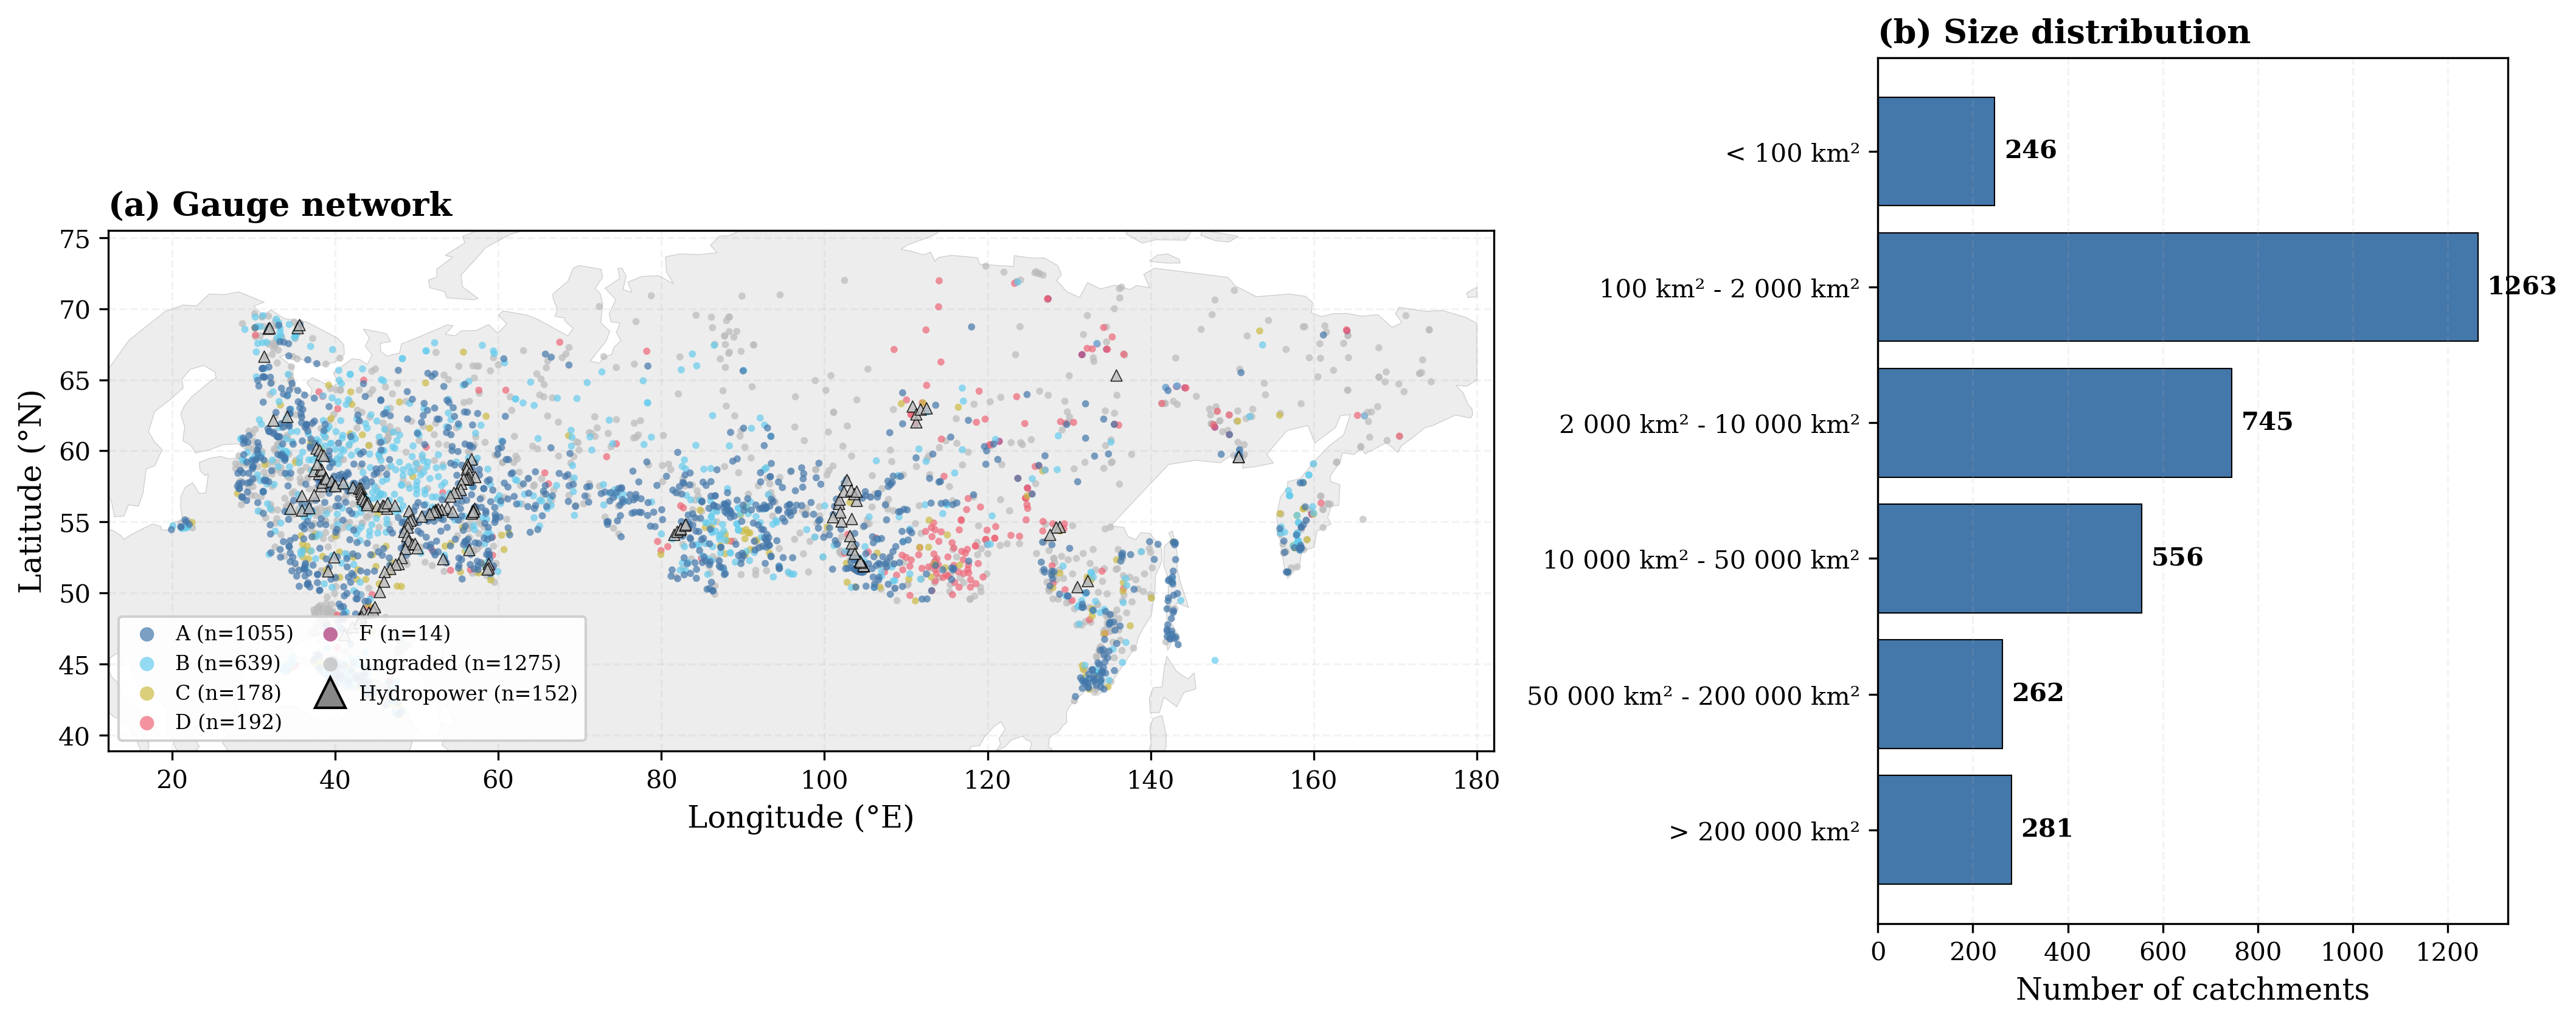
\includegraphics[width=0.95\columnwidth]{../images/fig_gauge_network.png}
\caption{(a) Spatial distribution of \ntotal gauging stations colored by discharge quality grade (A--F; triangles denote hydropower stations). (b) Catchment size distribution. Higher gauge density in European Russia and southern Siberia reflects Roshydromet's operational network.}
\label{fig:gauge_network}
\end{figure}

\section{Data Sources and Methods}
\label{sec:data_sources_methods}

\subsection{Hydrological Data: AIS GMVO}
\subsubsection{Data Source and Selection Criteria}
Daily discharge and water level observations were obtained from the Automated Information System of State Monitoring of Water Bodies (AIS GMVO), operated by Roshydromet~\citep{AIS_GMVO}.
The database provides stage-discharge records for approximately 3000 active gauging stations across Russia.
The final dataset includes \ndischarge discharge gauging stations and \nwaterlevel water level gauges across \ntotal delineated watersheds.
Selection criteria:
\begin{itemize}
    \item Minimum 10 years of available records between \years
    \item Data completeness $>$80\% during the study period for high-quality subset (\nhighquality gauges)
    \item Quality flags indicating operational sensors and regular maintenance
\end{itemize}

Quality tiers are assigned by the automated grading procedure described below: \emph{decent quality} gauges receive overall grades A--C; the \emph{high-quality} subset comprises Grade~A gauges ($\geq$95\% completeness, $\leq$2 minor flags).
Overall, 86\% of discharge gauges meet the decent quality threshold, with the high-quality subset comprising \nhighquality gauges (detailed data organization in Sect.~\ref{sec:data_records}).

The \years period was selected because systematic digitization and standardized reporting procedures were implemented across Roshydromet's network during this era.

\subsubsection{Quality Control}
Each discharge time series was assessed through a quality control procedure operating at annual (hydrological year) resolution.
The procedure evaluates four categories of quality metrics:

\begin{enumerate}
    \item \textbf{Anomaly detection:} Outliers flagged when values exceed 8 robust standard deviations (median absolute deviation, MAD~$\times$~1.4826) from a 30-day centered rolling median. The 8$\sigma$ threshold (vs.\ the more common 3--5$\sigma$) avoids flagging genuine flood peaks, which can exceed 20$\times$ median discharge during spring snowmelt. Constant-value periods ($>$30 consecutive days) flagged separately. Negative discharge values rejected.
    \item \textbf{Climatology checks:} Each year compared against a day-of-year climatology (mean across all years). Metrics include Pearson correlation with climatology, normalized RMSE, and amplitude ratio (peak discharge / climatological peak). For catchments with seasonal flow regimes (75th-percentile peak ratio $\geq$10), years with peak ratio $<$30\% of the gauge's 75th-percentile peak ratio are flagged as critical failures, targeting sensor malfunction rather than genuine low-flow years. Stable-regime catchments are exempted from this check.
    \item \textbf{Meteorological response:} Precipitation events ($>$5~mm/day) are matched against discharge response within a 7-day window (10\% increase threshold). Cross-correlation between daily $P$ and $Q$ computed at lags 0--14 days to identify the dominant response time. The Richards--Baker flashiness index quantifies flow variability. Thresholds are set conservatively low (cross-correlation $>$0.1, event response rate $>$20\%) to avoid penalizing snowmelt-dominated catchments where precipitation--discharge coupling is inherently weak.
    \item \textbf{Gap-filling:} Gaps $\leq$6 days interpolated using second-order polynomial interpolation; longer gaps retained as missing. Interpolated values producing negative discharge set to missing.
\end{enumerate}

Each year receives a grade (A--F, no E) based on 18 quality flags of varying severity (critical, major, minor): any critical flag assigns F; $\geq$2 major flags or completeness $<$70\% assigns D; 1 major flag or $\geq$5 minor flags assigns C; 3--4 minor flags assigns B; $\leq$2 minor flags with completeness $\geq$95\% assigns A.
Gauge-level grades aggregate year-level results, capped by the fraction of usable years: usable fraction $<$50\% caps at D, $<$70\% caps at C.
Gauges with overall grade A--C are classified as \emph{decent quality} (86\% of discharge gauges); grades D--F as \emph{poor}.

Discharge was standardized to mm/day by dividing volumetric flow (m$^3$\,s$^{-1}$) by catchment area.

\subsubsection{Water Level Processing}
Daily water level records (\nwaterlevel gauges, including 152 hydropower and reservoir gauges) were parsed from AIS GMVO exports with the following QC:
zero values (instrument artifacts) were replaced with day-of-year medians computed from non-zero observations at the same gauge;
gaps $\leq$6 days were interpolated using second-order polynomial interpolation (reservoir gauges: $\leq$15 days);
multi-source records for the same gauge were merged using preferential selection (latest correction takes precedence).
All water levels are in centimetres, referenced to the Baltic Sea datum as reported in AIS GMVO metadata.
No automated quality grading (A--F) was applied to water level data; users should assess completeness per gauge before use.

\begin{figure}[htbp]
\centering
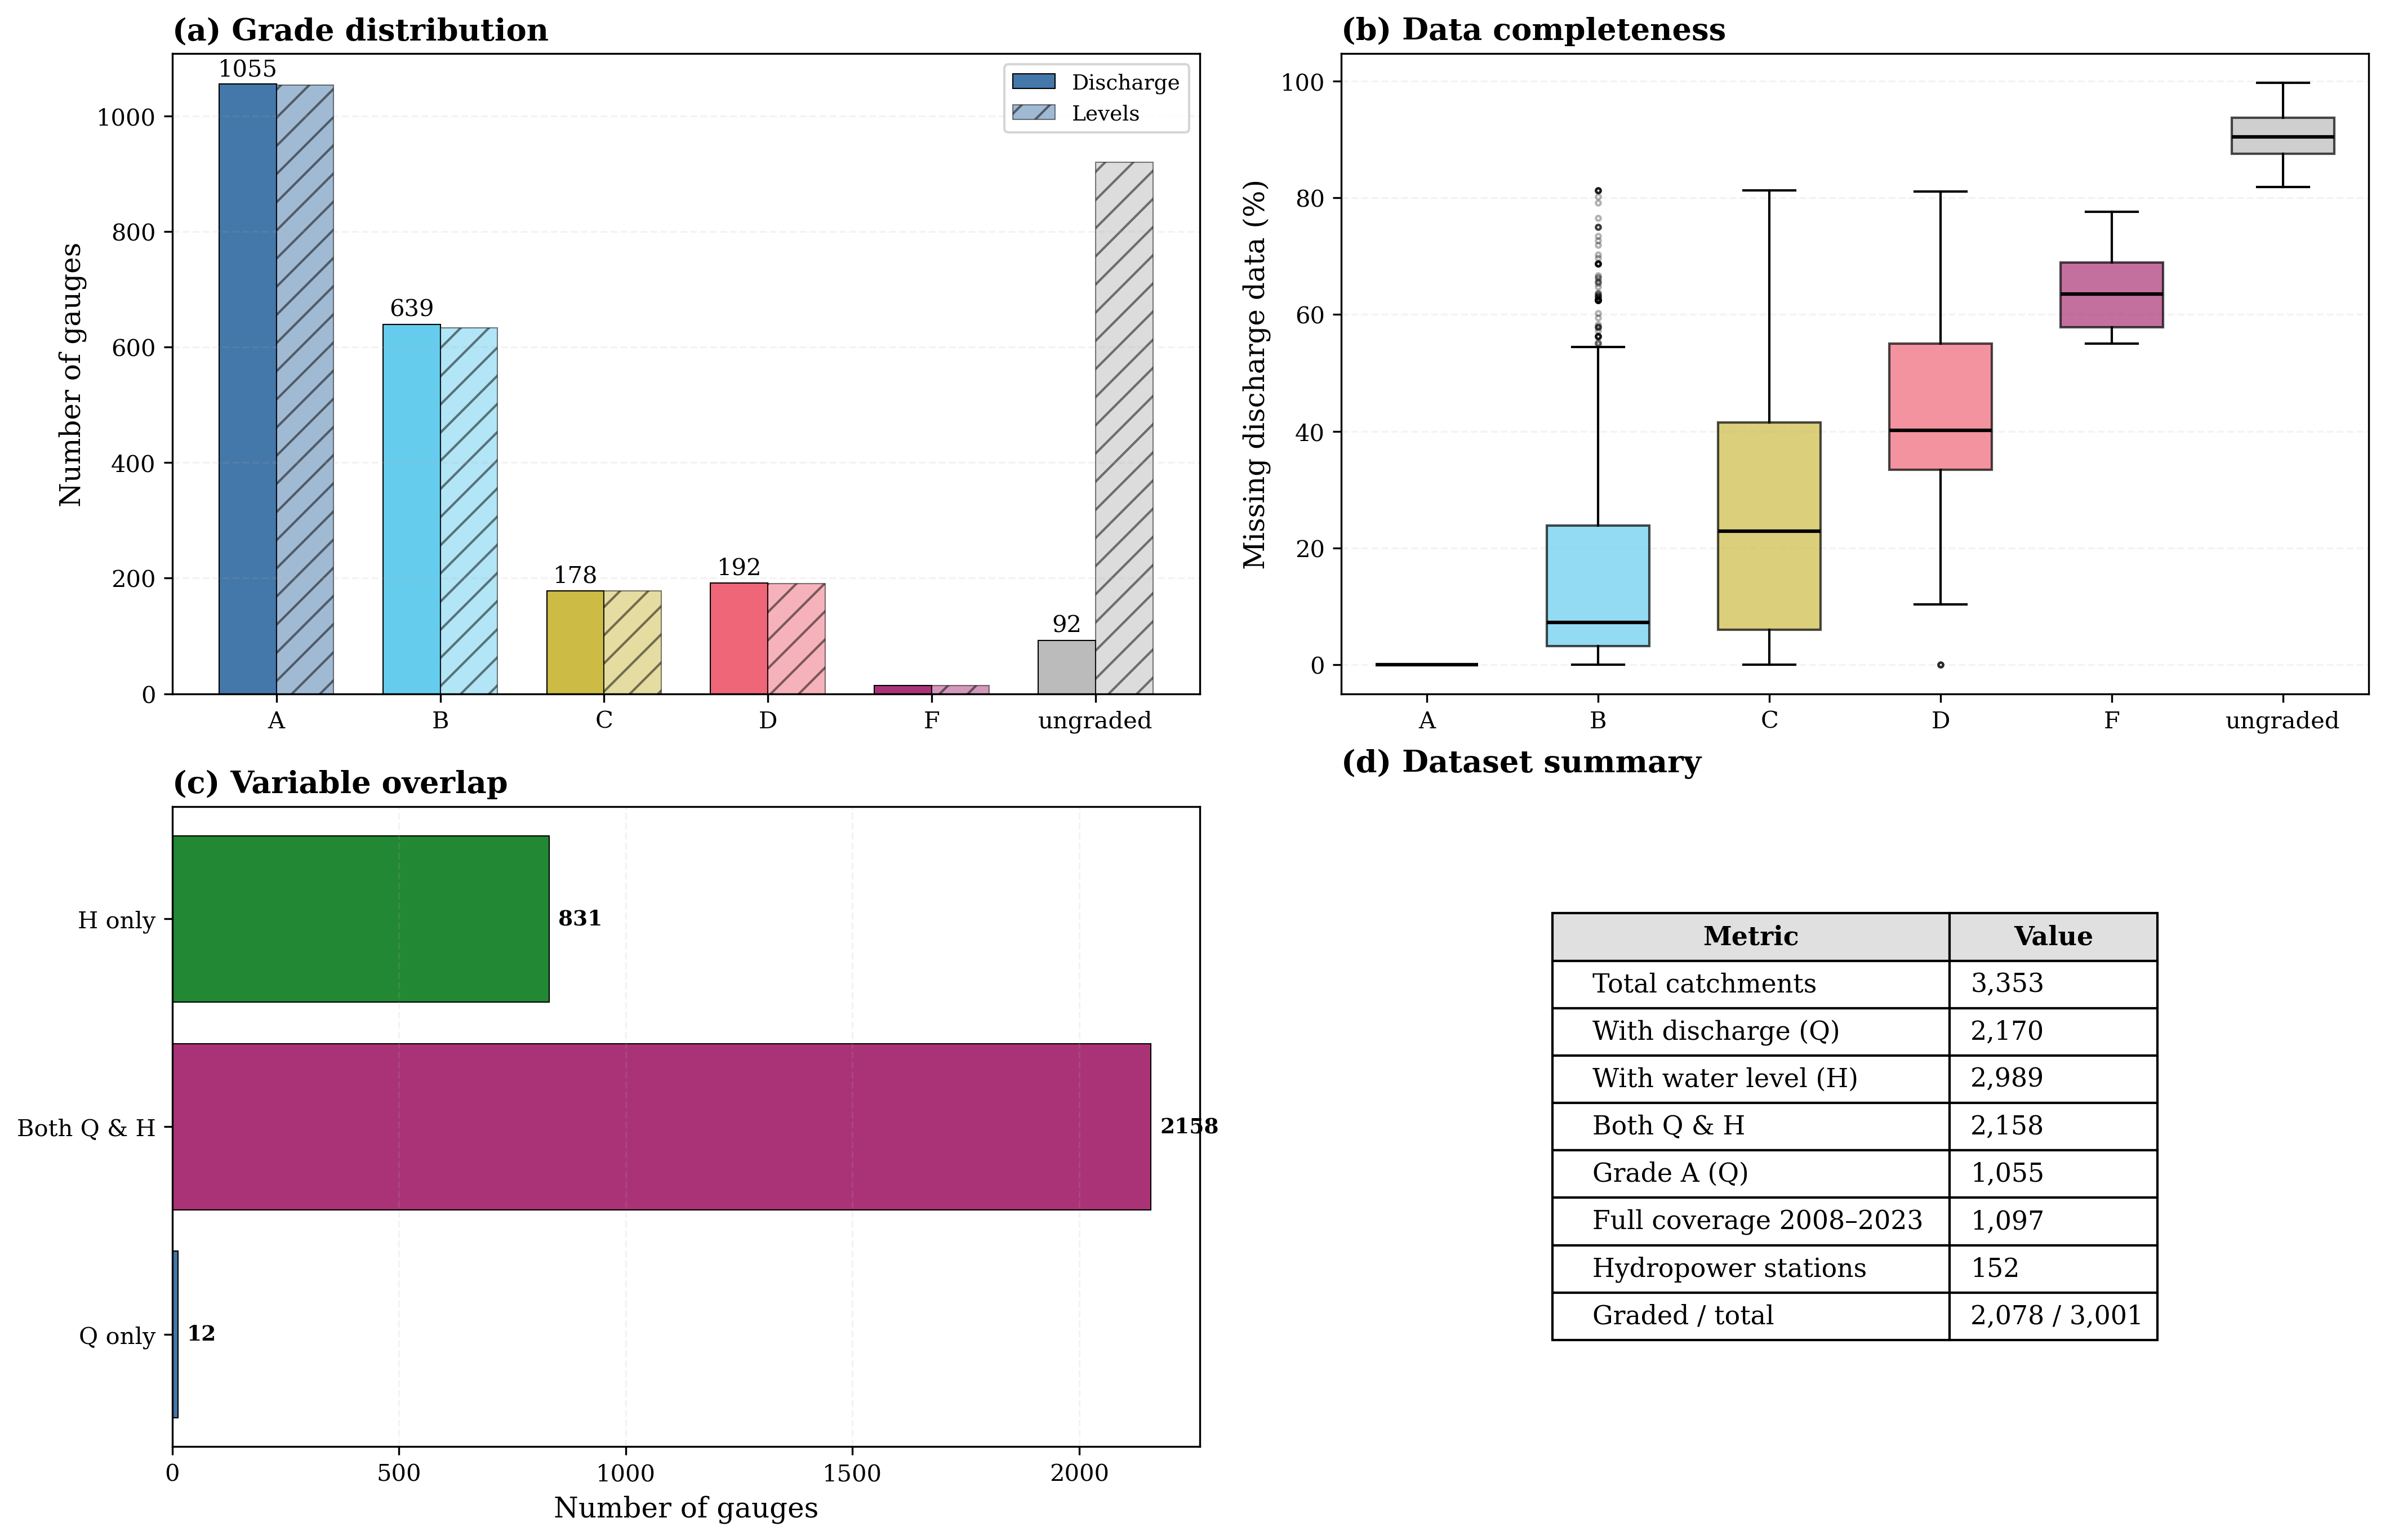
\includegraphics[width=0.95\columnwidth]{../images/fig_quality_assessment.png}
\caption{Quality assessment summary for the CAMELS-RU discharge network: data completeness, quality grade distribution, and temporal coverage across the \years study period.}
\label{fig:quality_assessment}
\end{figure}

\begin{figure}[htbp]
\centering
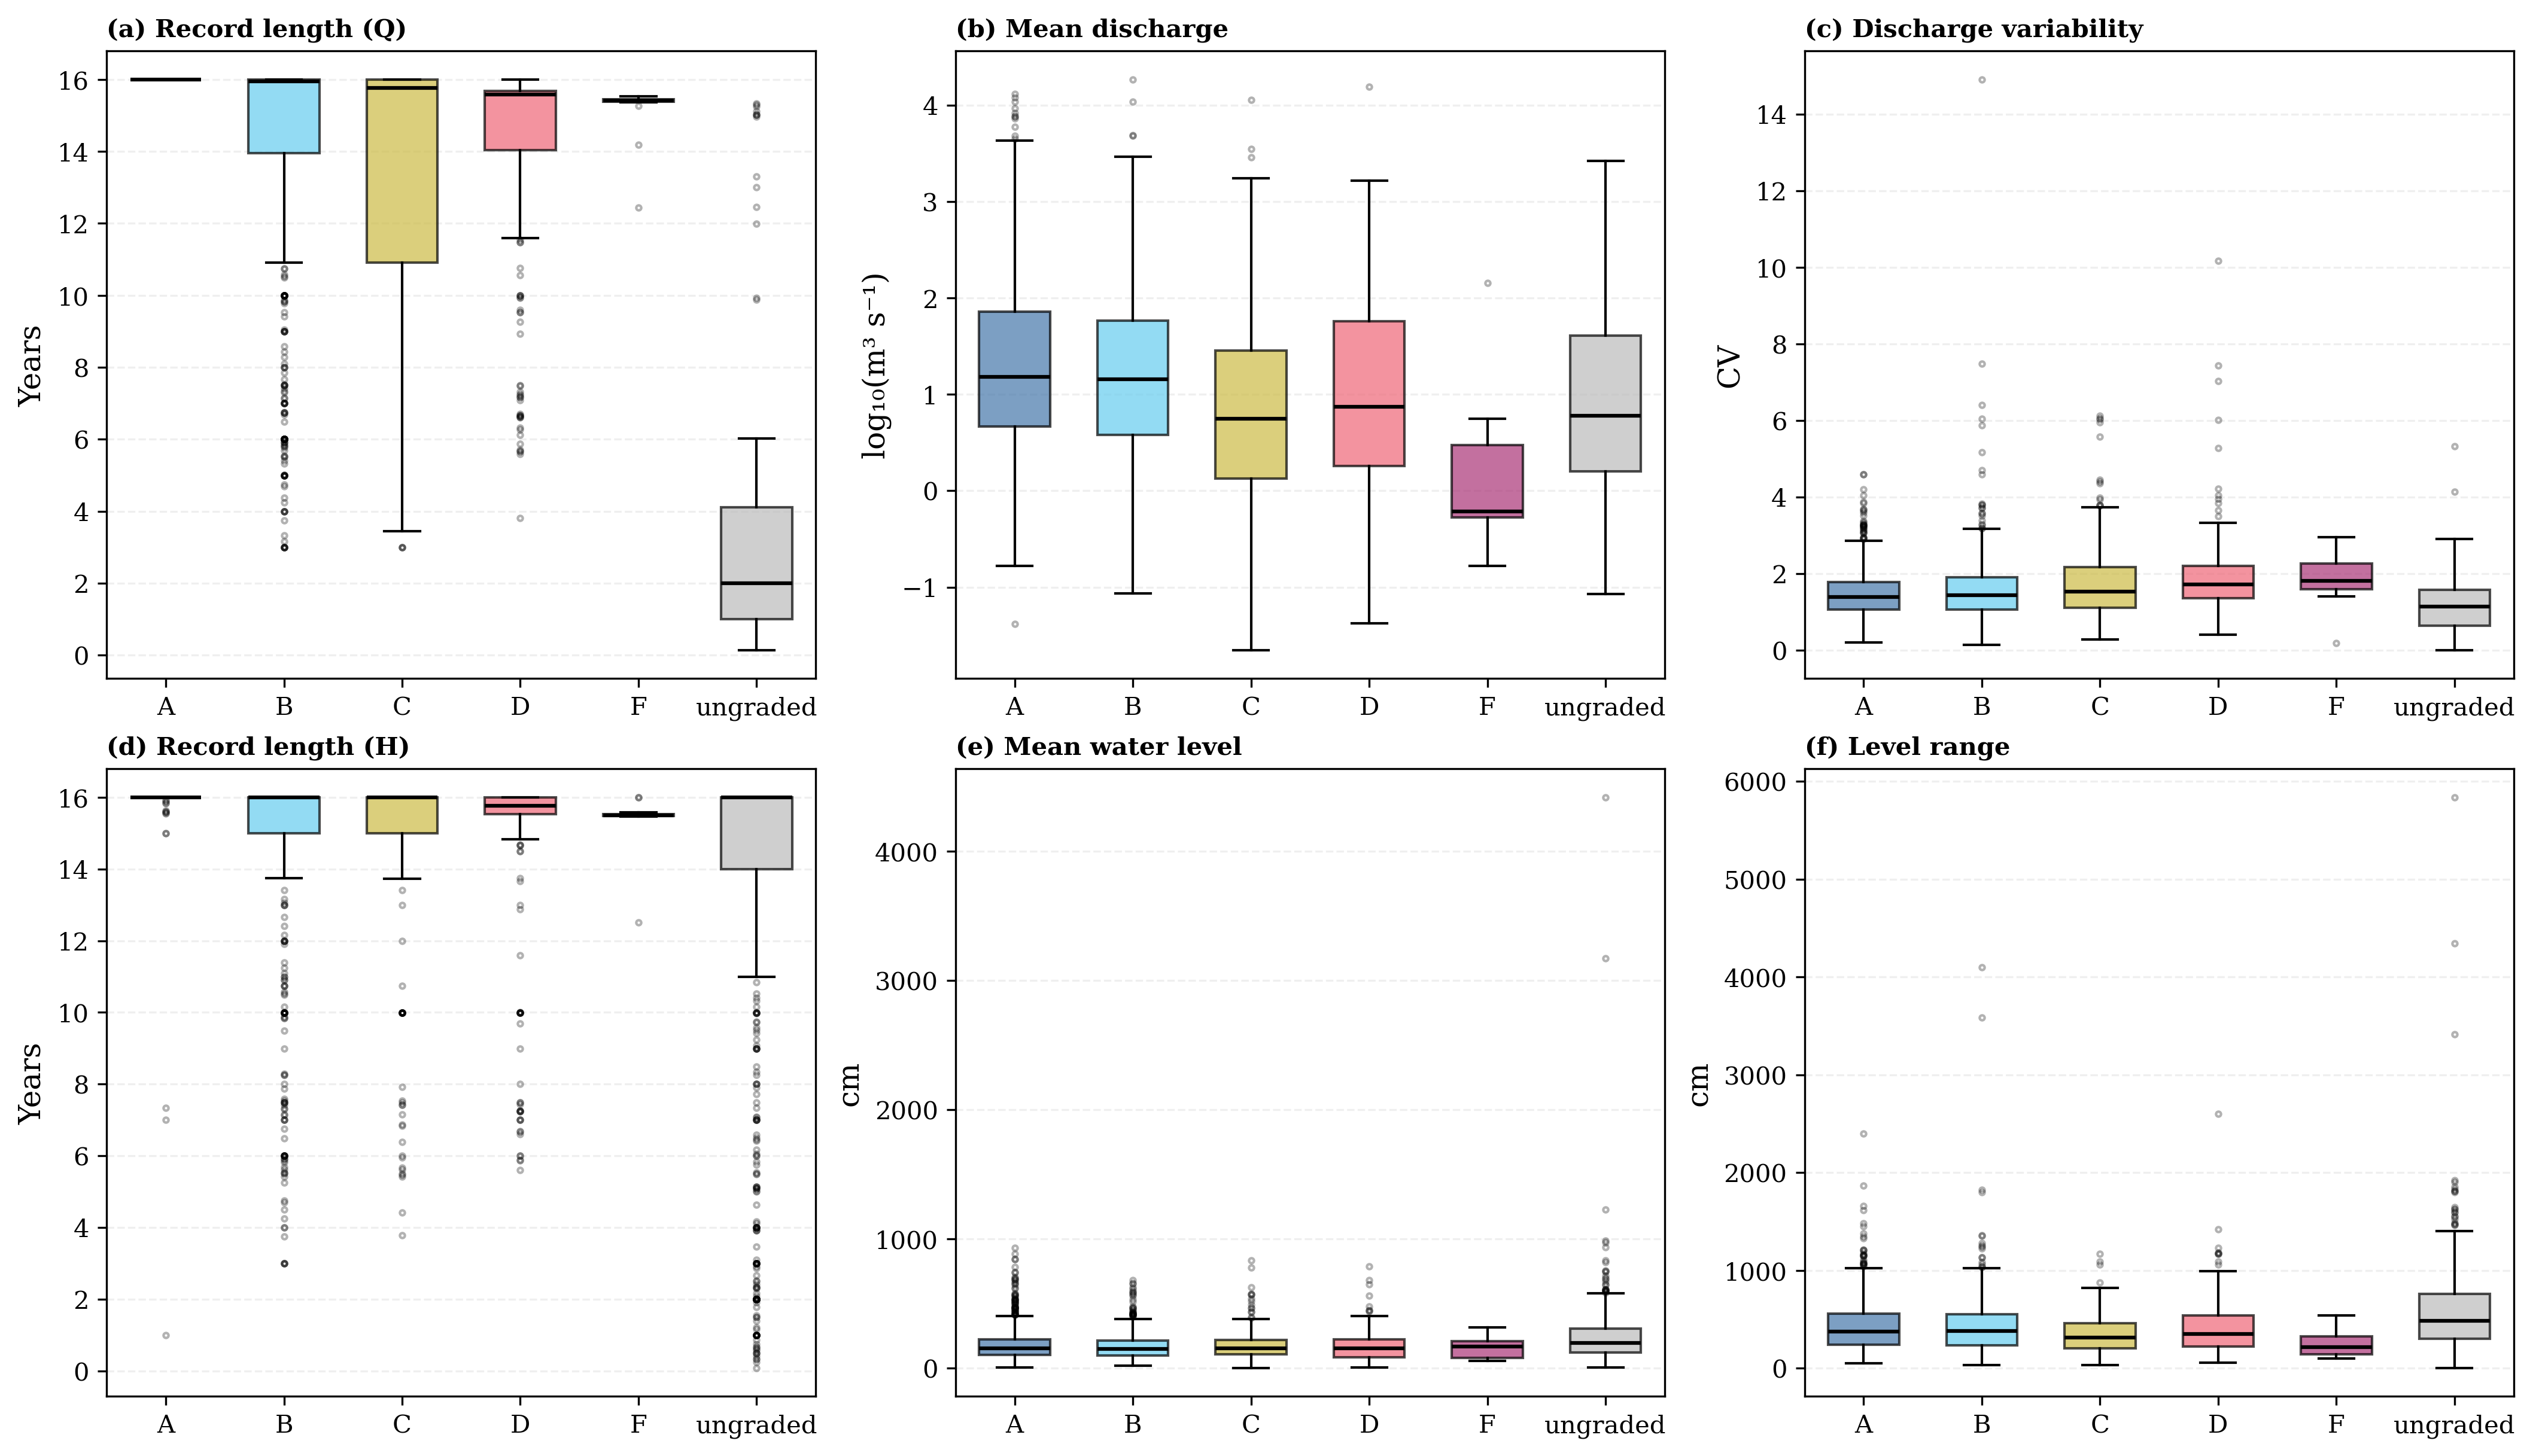
\includegraphics[width=0.95\columnwidth]{../images/fig_hydro_characteristics.png}
\caption{Discharge and water level characteristics across quality grades: summary statistics for the \ndischarge discharge gauges and \nwaterlevel water level gauges.}
\label{fig:hydro_characteristics}
\end{figure}

\subsection{Meteorological Forcing Data}
\subsubsection{ERA5-Land Reanalysis}
Meteorological forcing derived from ERA5-Land reanalysis~\citep{Munoz2021}, providing 0.1$^\circ$ ($\sim$9~km) hourly data aggregated to daily resolution.
Variables extracted:
\begin{itemize}
    \item Air temperature: mean, minimum, maximum ($^\circ$C)
    \item Potential evapotranspiration (mm/day, computed via Penman-Monteith)
    \item Precipitation (mm/day): mean annual \erafiveannual across catchments
\end{itemize}

For each catchment, basin-averaged forcing computed by weighting ERA5-Land grid cells by fractional catchment coverage, applying the standard environmental lapse rate ($-6.5^\circ$C/km) for elevation correction in mountain basins.

\subsubsection{MSWEP Precipitation}
Precipitation data sourced from Multi-Source Weighted-Ensemble Precipitation (MSWEP) version 2.8~\citep{Beck2019MSWEP}, a global precipitation dataset merging gauge observations, satellite estimates, and reanalysis data at 0.1$^\circ$ resolution.
Mean annual precipitation: \mswepannual across CAMELS-RU catchments.
MSWEP outperforms reanalysis-only products in gauge-sparse and snowfall-dominated regions~\citep{Beck2017MSWEP}.
Daily precipitation (mm/day) aggregated to catchment scale using area-weighted averaging of grid cells intersecting each watershed boundary.

\subsubsection{Inter-Dataset Validation}
Three precipitation products (ERA5-Land, MSWEP, GPCP) were cross-validated to assess forcing reliability.
Daily correlations range from $r = \eragpcpcorr$ (ERA5-Land vs.\ GPCP) to $r = \eramsweprcorr$ (ERA5-Land vs.\ MSWEP), with systematic differences in annual totals reflecting different data sources and spatial resolutions (see Sect.~\ref{sec:technical_validation}).

\subsection{Watershed Boundaries: Manual Verification}
\subsubsection{Base Delineation}
Initial catchment boundaries delineated using the MERIT Hydro digital elevation model (DEM;~\citealt{Yamazaki2019}) (3-arcsecond, $\sim$90~m resolution globally) and associated flow direction/accumulation grids.
MERIT Hydro reduces elevation errors in flat and forested terrain compared to earlier global DEMs by incorporating satellite altimetry and river network constraints.

Automated pour-point snapping algorithm identified nearest high-accumulation pixel (upstream area within 5\% of gauge catchment area reported by Roshydromet) within 500~m search radius of gauge coordinates.
Watershed delineation performed using standard D8 flow routing algorithm.

\subsubsection{Manual Expert Verification}
Every watershed boundary (\ntotal catchments) was manually verified and adjusted by a hydrographic expert using:
\begin{itemize}
    \item High-resolution satellite imagery (Google Earth, Sentinel-2 10~m)
    \item MERIT Hydro river network overlay
    \item Official Roshydromet topographic maps (1:100,000 scale)
    \item Local terrain knowledge and hydrographic principles
\end{itemize}

Manual adjustments corrected:
\begin{itemize}
    \item DEM artifacts in flat terrain (West Siberian Lowland, river deltas)
    \item Flow direction errors at confluences and braided reaches
    \item Canal diversions and reservoirs altering natural drainage
    \item Karst hydrology and subsurface flow contributions
\end{itemize}

\subsubsection{Validation Against Official Data}
Comparison with official Roshydromet catchment areas yielded:
\begin{itemize}
    \item Mean areal error: \meanerror (absolute difference)
    \item \withinfive of catchments within 5\% error
    \item \withinten of catchments within 10\% error
    \item Largest errors ($>$15\%) occur in complex karst terrain (Ural Mountains) and anthropogenically modified basins (irrigation canals, inter-basin transfers)
\end{itemize}

For comparison, \citet{Lehner2008} and \citet{Yamazaki2019} report 10--15\% mean areal errors from automated delineation in flat and permafrost terrain.

Known limitations of the dataset (temporal coverage, nested catchments, attribute temporal mismatch, and others) are consolidated in Sect.~\ref{sec:limitations}.

\subsection{Physiographic Attributes: HydroATLAS}
For each of the \ntotal manually verified catchment boundaries, all variables from the HydroATLAS v1.0 database~\citep{Linke2019} were extracted by spatially aggregating raster layers within watershed polygons using area-weighted averaging.
This produces 288 catchment-specific attribute values spanning hydrology, physiography, climate (including monthly temperature and precipitation), land cover, soil and geology, and anthropogenic variables.
The full attribute set is provided in the released CSV file.

Table~\ref{tab:hydroatlas_attributes} lists a recommended primary subset of \nattributes attributes selected by retaining upstream-aggregated annual variables and removing 12 features with pairwise $|r| > 0.7$ (e.g., slope correlated with elevation; aridity index redundant with precipitation and potential evapotranspiration, PET).
All removed attributes---including aridity index, slope, temperature, and soil properties---remain available in the full released attribute file for users who need them.

\begin{table*}[htbp]
\centering
\caption{Static catchment attributes derived from HydroATLAS v1.0 included in CAMELS-RU (\nattributes primary subset). Initial selection retained attributes matching upstream and sub-basin aggregation conventions; 12 inter-correlated features were subsequently removed (see Sect.~\ref{sec:data_sources_methods}). The full set of 288 HydroATLAS attributes is provided in the released CSV.}
\label{tab:hydroatlas_attributes}
\small
\begin{threeparttable}
\begin{tabular}{lllp{7cm}}
\toprule
\textbf{Category} & \textbf{Attribute} & \textbf{Unit} & \textbf{Description} \\
\midrule
\multirow{5}{*}{Climate \& water balance}
& ele\_mt\_uav & m & Mean elevation \\
& pre\_mm\_uyr & mm/yr & Mean annual precipitation \\
& pet\_mm\_uyr & mm/yr & Mean annual potential evapotranspiration \\
& aet\_mm\_uyr & mm/yr & Mean annual actual evapotranspiration \\
& snw\_pc\_uyr & \% & Mean annual snow cover extent \\
\midrule
\multirow{5}{*}{Land cover}
& for\_pc\_use & \% & Forest cover \\
& crp\_pc\_use & \% & Cropland cover \\
& pst\_pc\_use & \% & Pasture/grassland cover \\
& ire\_pc\_use & \% & Irrigated area \\
& pac\_pc\_use & \% & Protected area coverage \\
\midrule
\multirow{2}{*}{Cryosphere}
& gla\_pc\_use & \% & Glacier cover \\
& prm\_pc\_use & \% & Permafrost extent \\
\midrule
\multirow{3}{*}{Soil}
& cly\_pc\_uav & \% & Clay content (mean) \\
& slt\_pc\_uav & \% & Silt content (mean) \\
& snd\_pc\_uav & \% & Sand content (mean) \\
\midrule
\multirow{2}{*}{Hydrogeology}
& gwt\_cm\_sav & cm & Groundwater table depth \\
& kar\_pc\_use & \% & Karst area extent \\
\midrule
\multirow{2}{*}{Water bodies}
& inu\_pc\_ult & \% & Inundation extent \\
& lka\_pc\_use & \% & Lake/reservoir area \\
\midrule
\multirow{3}{*}{Human impact}
& ppd\_pk\_uav & pers/km$^2$ & Population density \\
& urb\_pc\_use & \% & Urban/built-up area \\
& gdp\_ud\_sav & USD/km$^2$ & GDP density \\
\bottomrule
\end{tabular}
\begin{tablenotes}
\small
\item All attributes are watershed-level aggregates computed individually for each manually verified catchment boundary using area-weighted spatial averaging.
\item Attribute codes follow HydroATLAS naming: suffix indicates aggregation (uav = upstream area-weighted average, use = upstream spatial extent, uyr = upstream annual mean, sav = sub-basin average, ult = upstream ultimate).
\end{tablenotes}
\end{threeparttable}
\end{table*}


\subsection{Hydrological Signatures}
We computed \nsignatures hydrological signatures (Table~\ref{tab:hydro_signatures}) characterizing discharge magnitude, variability, timing, and extremes for gauges meeting the per-year completeness criterion ($>$70\% for at least 5 hydrological years; $N = \nsigngauges$, or $N = \nhalfflowgauges$ for half-flow date which requires $>$82\%), following established methodologies~\citep{Sawicz2011,McMillan2017}.

Signatures were computed separately for individual hydrological years (October--September) and then averaged to produce catchment-characteristic values.
Key methodological choices:
\begin{itemize}
    \item Runoff ratio uses ERA5-Land precipitation as denominator; ratios differ with MSWEP ($\sim$0.36) or GPCP ($\sim$0.33) due to lower annual totals
    \item Flow duration curve (FDC) slope computed as $[\ln(Q_{33}) - \ln(Q_{66})] / (66 - 33) \times 100$ where $Q_p$ is discharge at the $p$-th exceedance percentile; positive values indicate steeper curves (note: sign convention opposite to \citealt{Sawicz2011})
    \item Baseflow index (BFI) computed using an ensemble of 1{,}000 Lyne--Hollick digital filter~\citep{Nathan1990} runs with $\alpha \sim U[0.9, 0.98]$ (3-pass), following \citet{Euser2013}
    \item Half-flow date requires $>$82\% annual completeness ($\geq$300 days) because partial years can shift the cumulative midpoint
    \item Richards--Baker flashiness index: $\sum|Q_i - Q_{i-1}| / \sum Q_i$, dimensionless measure of day-to-day flow variability
    \item High-flow and low-flow durations: mean consecutive days above $2\times$ median (high) or below $0.2\times$ mean (low) discharge
\end{itemize}

\begin{table}[htbp]
\centering
\caption{Hydrological signatures computed for CAMELS-RU catchments. All signatures derived from daily discharge time series for gauges with $>$70\% data completeness per hydrological year and at least 5 qualifying years ($n = \nsigngauges$; half-flow date requires $>$82\% completeness, $n = \nhalfflowgauges$). FDC slope is positive for steeper curves (opposite sign convention to \citealt{Sawicz2011}).}
\label{tab:hydro_signatures}
\begin{tabular}{llp{5.5cm}}
\toprule
\textbf{Signature} & \textbf{Unit} & \textbf{Description} \\
\midrule
\multicolumn{3}{l}{\textit{Magnitude}} \\
\quad q\_mean & mm/day & Mean daily discharge \\
\quad runoff\_ratio & -- & Annual $Q/P$ ratio (ERA5-Land precipitation) \\
\midrule
\multicolumn{3}{l}{\textit{Variability}} \\
\quad q\_cv & -- & Coefficient of variation of daily discharge \\
\quad FDC\_slope & -- & FDC slope between 33rd and 66th exceedance percentiles (log-space; positive = steeper) \\
\quad flashiness\_index & -- & Richards--Baker index: $\sum|Q_{i}-Q_{i-1}|/\sum Q_i$ \\
\midrule
\multicolumn{3}{l}{\textit{Extremes}} \\
\quad Q5 & mm/day & 5th exceedance percentile (high flows) \\
\quad Q95 & mm/day & 95th exceedance percentile (low flows) \\
\quad high\_flow\_freq & \% of days & Days exceeding $2\times$ median discharge \\
\quad high\_flow\_dur & days & Mean duration of high-flow events ($>2\times$ median) \\
\midrule
\multicolumn{3}{l}{\textit{Baseflow}} \\
\quad baseflow\_index & -- & Baseflow fraction; ensemble of 1{,}000 Lyne--Hollick filter runs, $\alpha \sim U[0.9, 0.98]$, 3-pass \\
\midrule
\multicolumn{3}{l}{\textit{Low Flow}} \\
\quad low\_flow\_freq & \% of days & Days below $0.2\times$ mean discharge \\
\quad low\_flow\_dur & days & Mean duration of low-flow events ($<0.2\times$ mean) \\
\midrule
\multicolumn{3}{l}{\textit{Seasonality}} \\
\quad half\_flow\_date & day of hydro yr & Day of hydrological year (Oct~1 = day~1) when 50\% of annual streamflow volume has passed \\
\bottomrule
\end{tabular}
\end{table}




\section{Technical Validation}
\label{sec:technical_validation}

\subsection{Precipitation Dataset Intercomparison}

\subsubsection{Inter-Dataset Correlations}
Daily precipitation time series from three global products (ERA5-Land, MSWEP v2.8, GPCP v3.2) show agreement across \ntotal catchments:
\begin{itemize}
    \item ERA5-Land vs.\ MSWEP: spatial mean $r = \eramsweprcorr$ (s.d.\ $= 0.08$ across $n = \ntotal$ catchments), mean bias $-0.10$~mm/day
    \item ERA5-Land vs.\ GPCP: spatial mean $r = \eragpcpcorr$ (s.d.\ $= 0.10$), mean bias $+0.05$~mm/day
    \item MSWEP vs.\ GPCP: spatial mean $r = \mswepgpcpcorr$ (s.d.\ $= 0.09$), mean bias $+0.15$~mm/day
\end{itemize}
All correlations computed on daily time series ($p \ll 0.001$ for all catchments given $>$5000 daily pairs per gauge).

ERA5-Land and MSWEP show the highest daily agreement ($r = \eramsweprcorr$); correlations with GPCP are lower ($r = \eragpcpcorr$ to $\mswepgpcpcorr$), likely reflecting GPCP's coarser resolution (0.5$^\circ$ vs.\ 0.1$^\circ$) and different source data.
However, systematic biases in annual totals reflect different data assimilation approaches:

\begin{center}
\begin{tabular}{lccc}
\toprule
Dataset & Mean (mm/yr) & Std (mm/yr) & CV (\%) \\
\midrule
ERA5-Land & \erafiveannual & 121.7 & 13.6 \\
MSWEP & \mswepannual & 92.4 & 15.3 \\
GPCP & \gpcpannual & 96.9 & 14.8 \\
\bottomrule
\end{tabular}
\end{center}

ERA5-Land precipitation (\erafiveannual) exceeds MSWEP (\mswepannual) by $\sim$220~mm/yr (36\%; per-catchment mean bias $\sim$229~mm/yr).
ERA5 precipitation is a model forecast product, and its prognostic cloud microphysics scheme tends to overestimate snowfall at high latitudes~\citep{Wang2019,Lavers2022} (Figure~\ref{fig:precip_comparison}).
GPCP (\gpcpannual) is closer to MSWEP, suggesting ERA5-Land is the outlier.

\begin{figure}[htbp]
\centering
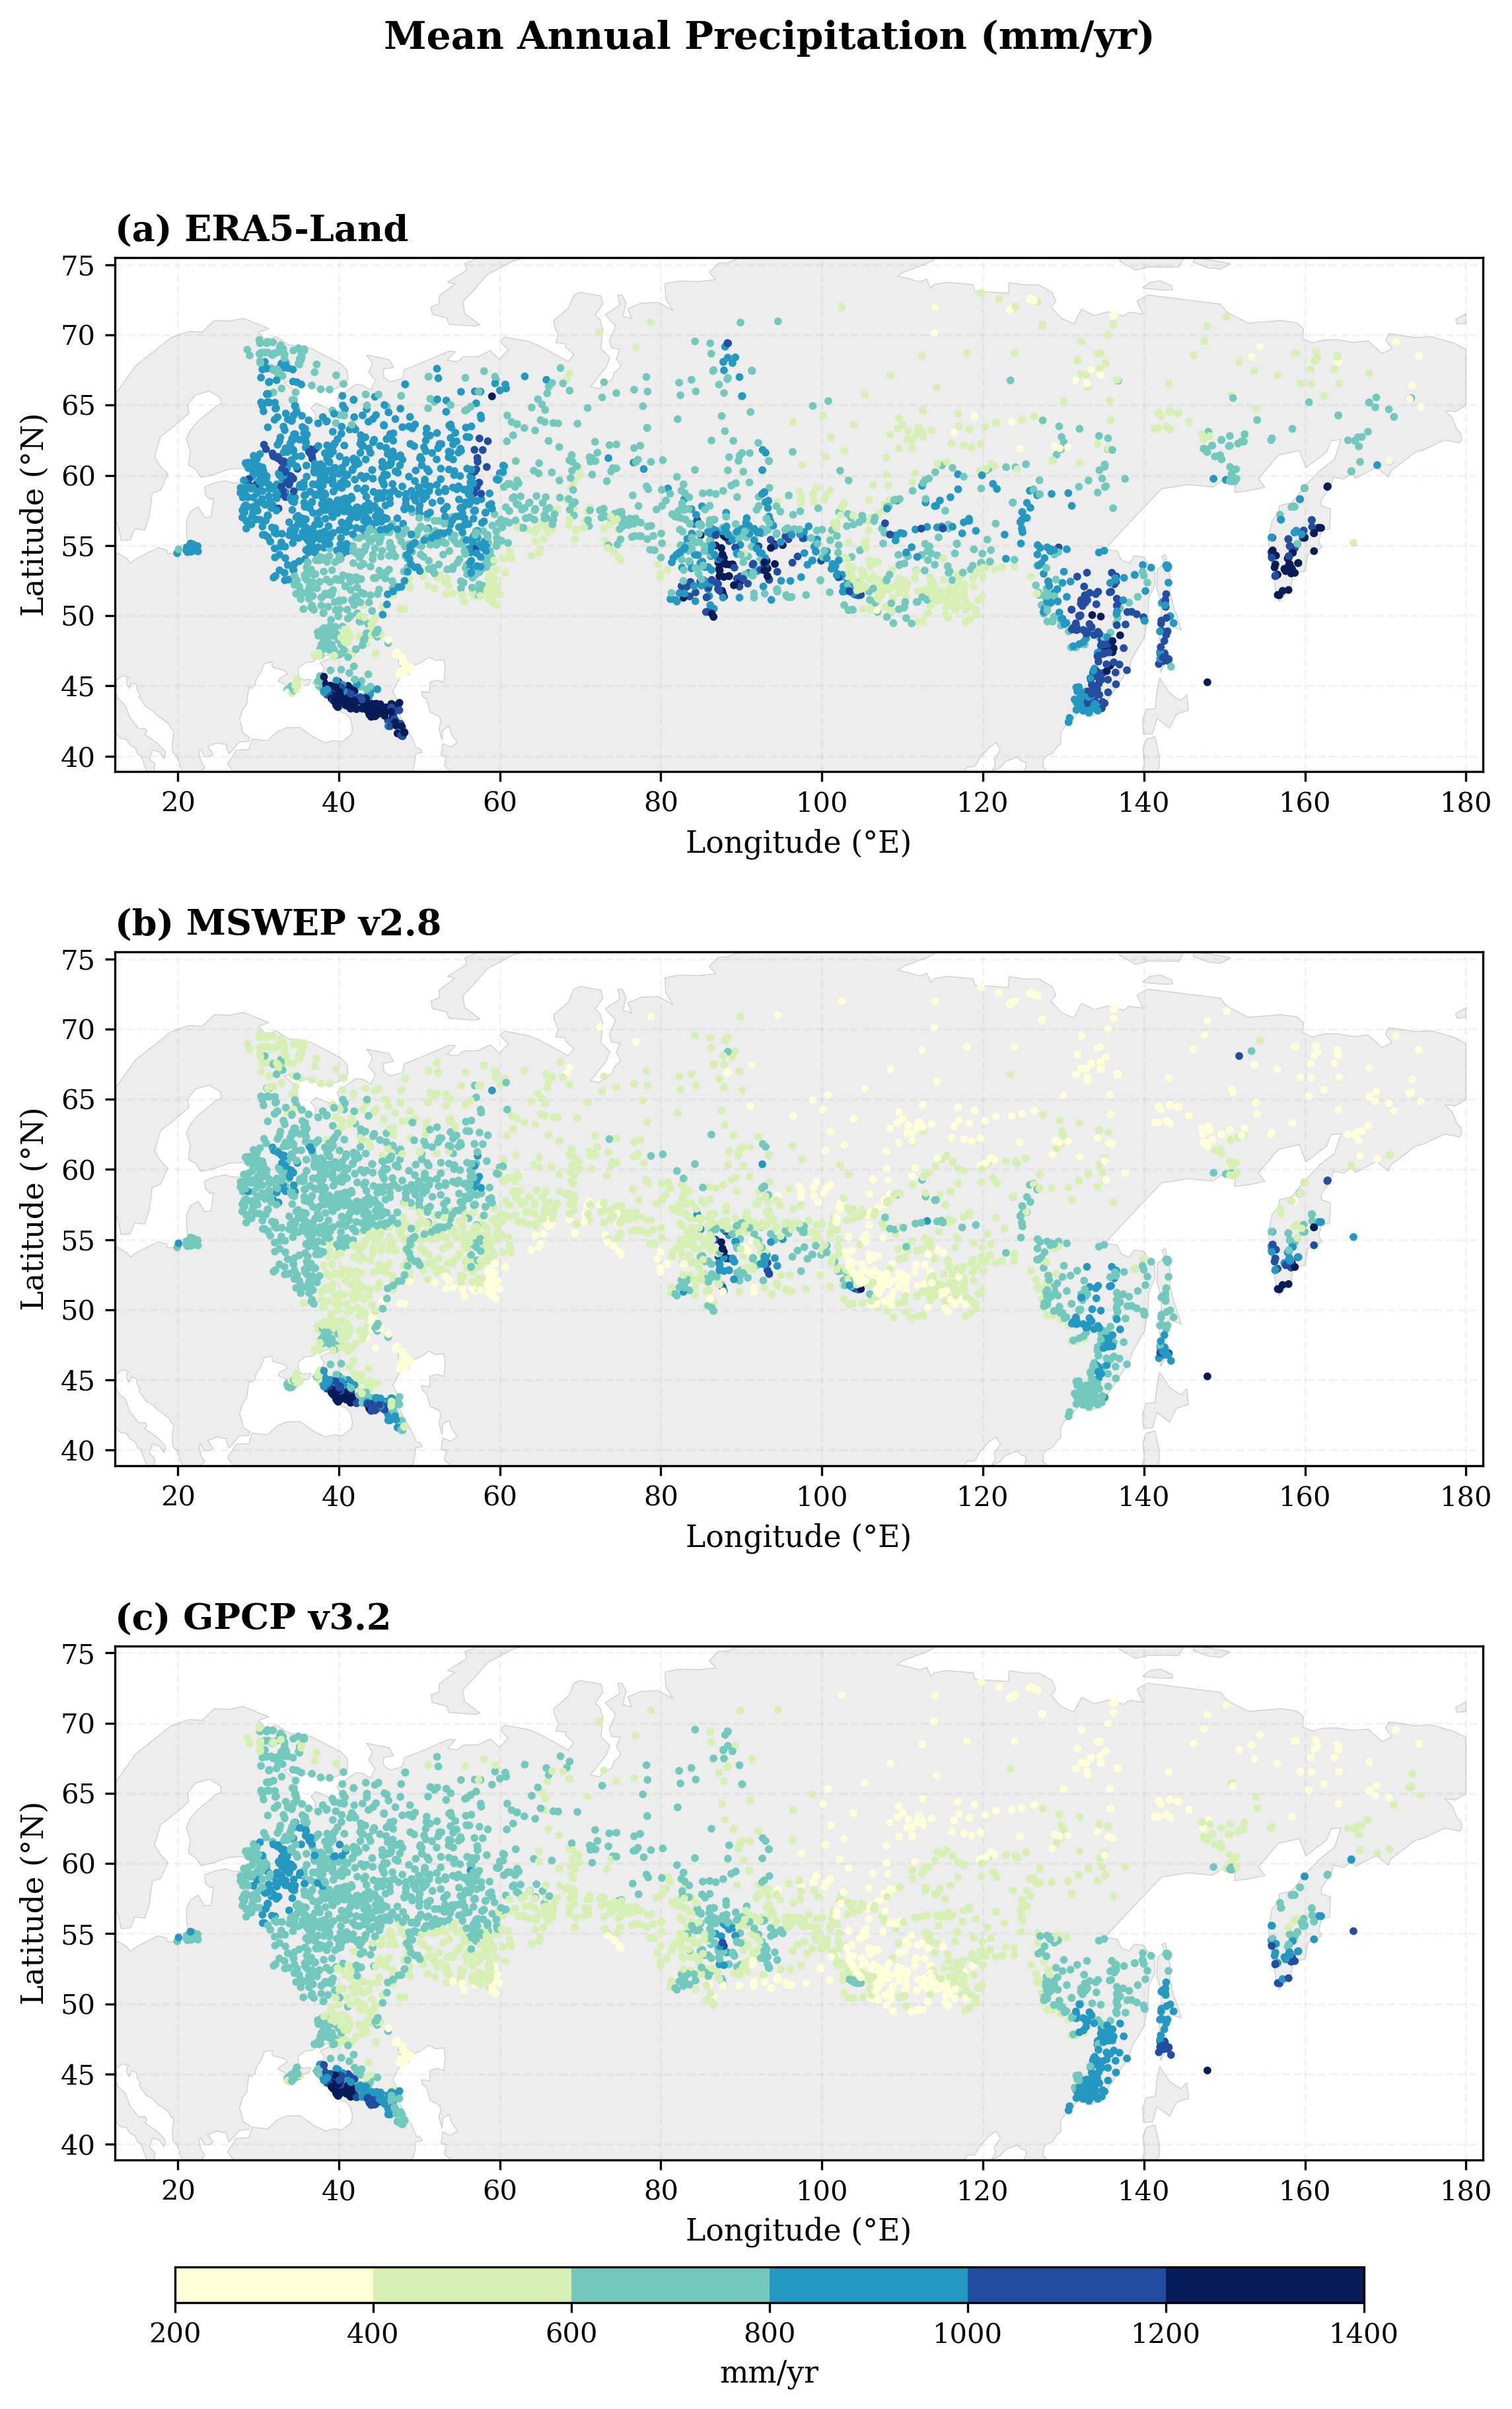
\includegraphics[width=0.95\columnwidth]{../images/fig_precip_comparison.png}
\caption{Spatial distribution of mean annual precipitation from three global products (ERA5-Land, MSWEP v2.8, GPCP v3.2) across CAMELS-RU catchments. ERA5-Land shows systematically higher values, particularly in mountainous and northern regions.}
\label{fig:precip_comparison}
\end{figure}

\begin{figure}[htbp]
\centering
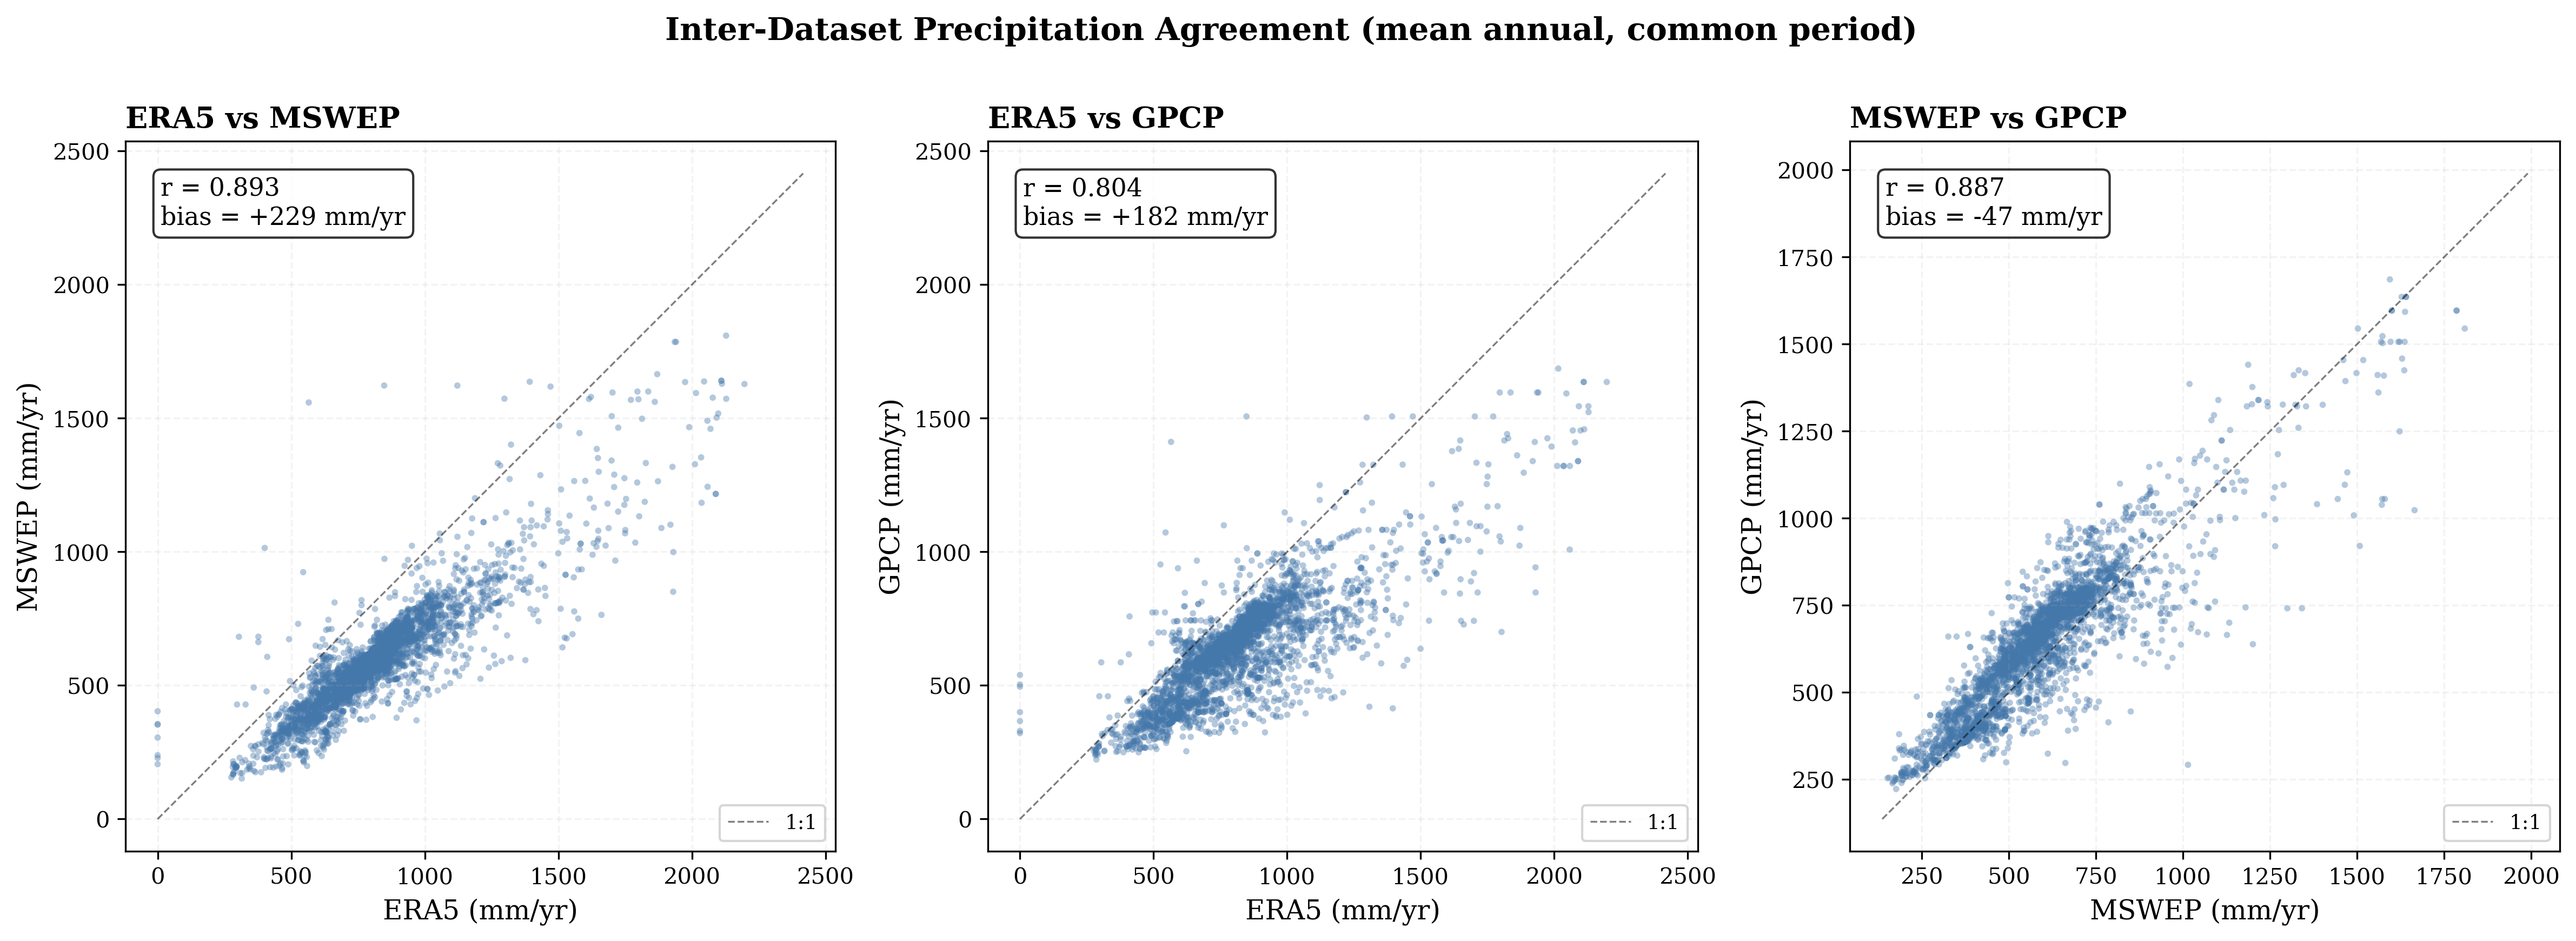
\includegraphics[width=0.95\columnwidth]{../images/fig_forcing_correlations.png}
\caption{Inter-dataset precipitation agreement: scatter plots of mean annual precipitation (mm/yr) for each catchment. Annotations show Pearson $r$ and mean bias for the annual values. Note that daily correlations (reported in text) differ from these annual correlations.}
\label{fig:forcing_correlations}
\end{figure}

\subsubsection{Water Balance Consistency}
Runoff ratios ($Q/P$) provide a consistency check on precipitation products through water balance closure.
ERA5-Land inherits ERA5 precipitation, which is generated by model physics rather than observation assimilation and tends to overestimate high-latitude snowfall~\citep{Wang2019}.
Because ERA5-Land supplies both precipitation and temperature/PET forcing, this analysis tests internal consistency rather than providing independent validation:

\begin{center}
\begin{tabular}{lccl}
\toprule
Dataset & Median $Q/P$ & Mean $Q/P$ & $Q/P > 1$ (\%) \\
\midrule
ERA5-Land & \medianrunoffratio & 0.278 & 0.0\% \checkmark \\
MSWEP & 0.361 & 0.420 & 5.1\% (87 gauges) \\
GPCP & 0.329 & 0.329 & 0.9\% (15 gauges) \\
\bottomrule
\end{tabular}
\end{center}

With ERA5-Land precipitation, all catchments yield $Q/P \leq 1$ (median \medianrunoffratio), consistent with an evapotranspiration proxy of 213~$\pm$~223~mm/yr (P$-$Q).
However, this partly reflects ERA5-Land's high-latitude wet bias rather than independent confirmation of discharge accuracy.
MSWEP produces $Q/P > 1$ for 5.1\% of catchments (87 gauges), which may indicate precipitation underestimation in high-discharge regions, watershed boundary errors, or unaccounted lateral flows.

Seasonal runoff ratios (ERA5-Land) reveal expected snowmelt dominance:
\begin{itemize}
    \item Winter (DJF): $Q/P = 0.15$ (snow storage phase)
    \item Spring (MAM): $Q/P = 0.48$ (snowmelt release, 3.2$\times$ winter)
    \item Summer (JJA): $Q/P = 0.18$ (high evapotranspiration)
    \item Autumn (SON): $Q/P = 0.25$ (declining ET, moderate flow)
\end{itemize}

\subsubsection{Precipitation--Discharge Relationship}
Linear regression of annual discharge vs.\ annual precipitation quantifies the marginal streamflow response to precipitation:
\begin{equation}
Q_{\text{annual}} = \alpha + \beta \times P_{\text{annual}}
\end{equation}

ERA5-Land yields a median slope $\beta = \climaticsensPQ$ (mean: 0.824), indicating that on average a 1~mm/yr increase in annual precipitation corresponds to a 0.824~mm/yr increase in discharge.
Note that $\beta$ is a simple regression slope, not the dimensionless precipitation elasticity of streamflow~\citep{Sankarasubramanian2001}; it depends on the absolute magnitudes of $P$ and $Q$.
The sub-unity slope is consistent with evapotranspiration buffering and storage changes that dampen the precipitation signal.
Only 0.7\% of catchments exceed $\beta = 1.0$, concentrated in karst terrain where groundwater imports from adjacent basins may supplement local precipitation inputs.

MSWEP yields $\beta = 1.07$ (14.2\% catchments $> 1$), which may reflect either precipitation underestimation or real differences in the precipitation--discharge relationship at lower annual totals.

\begin{figure}[htbp]
\centering
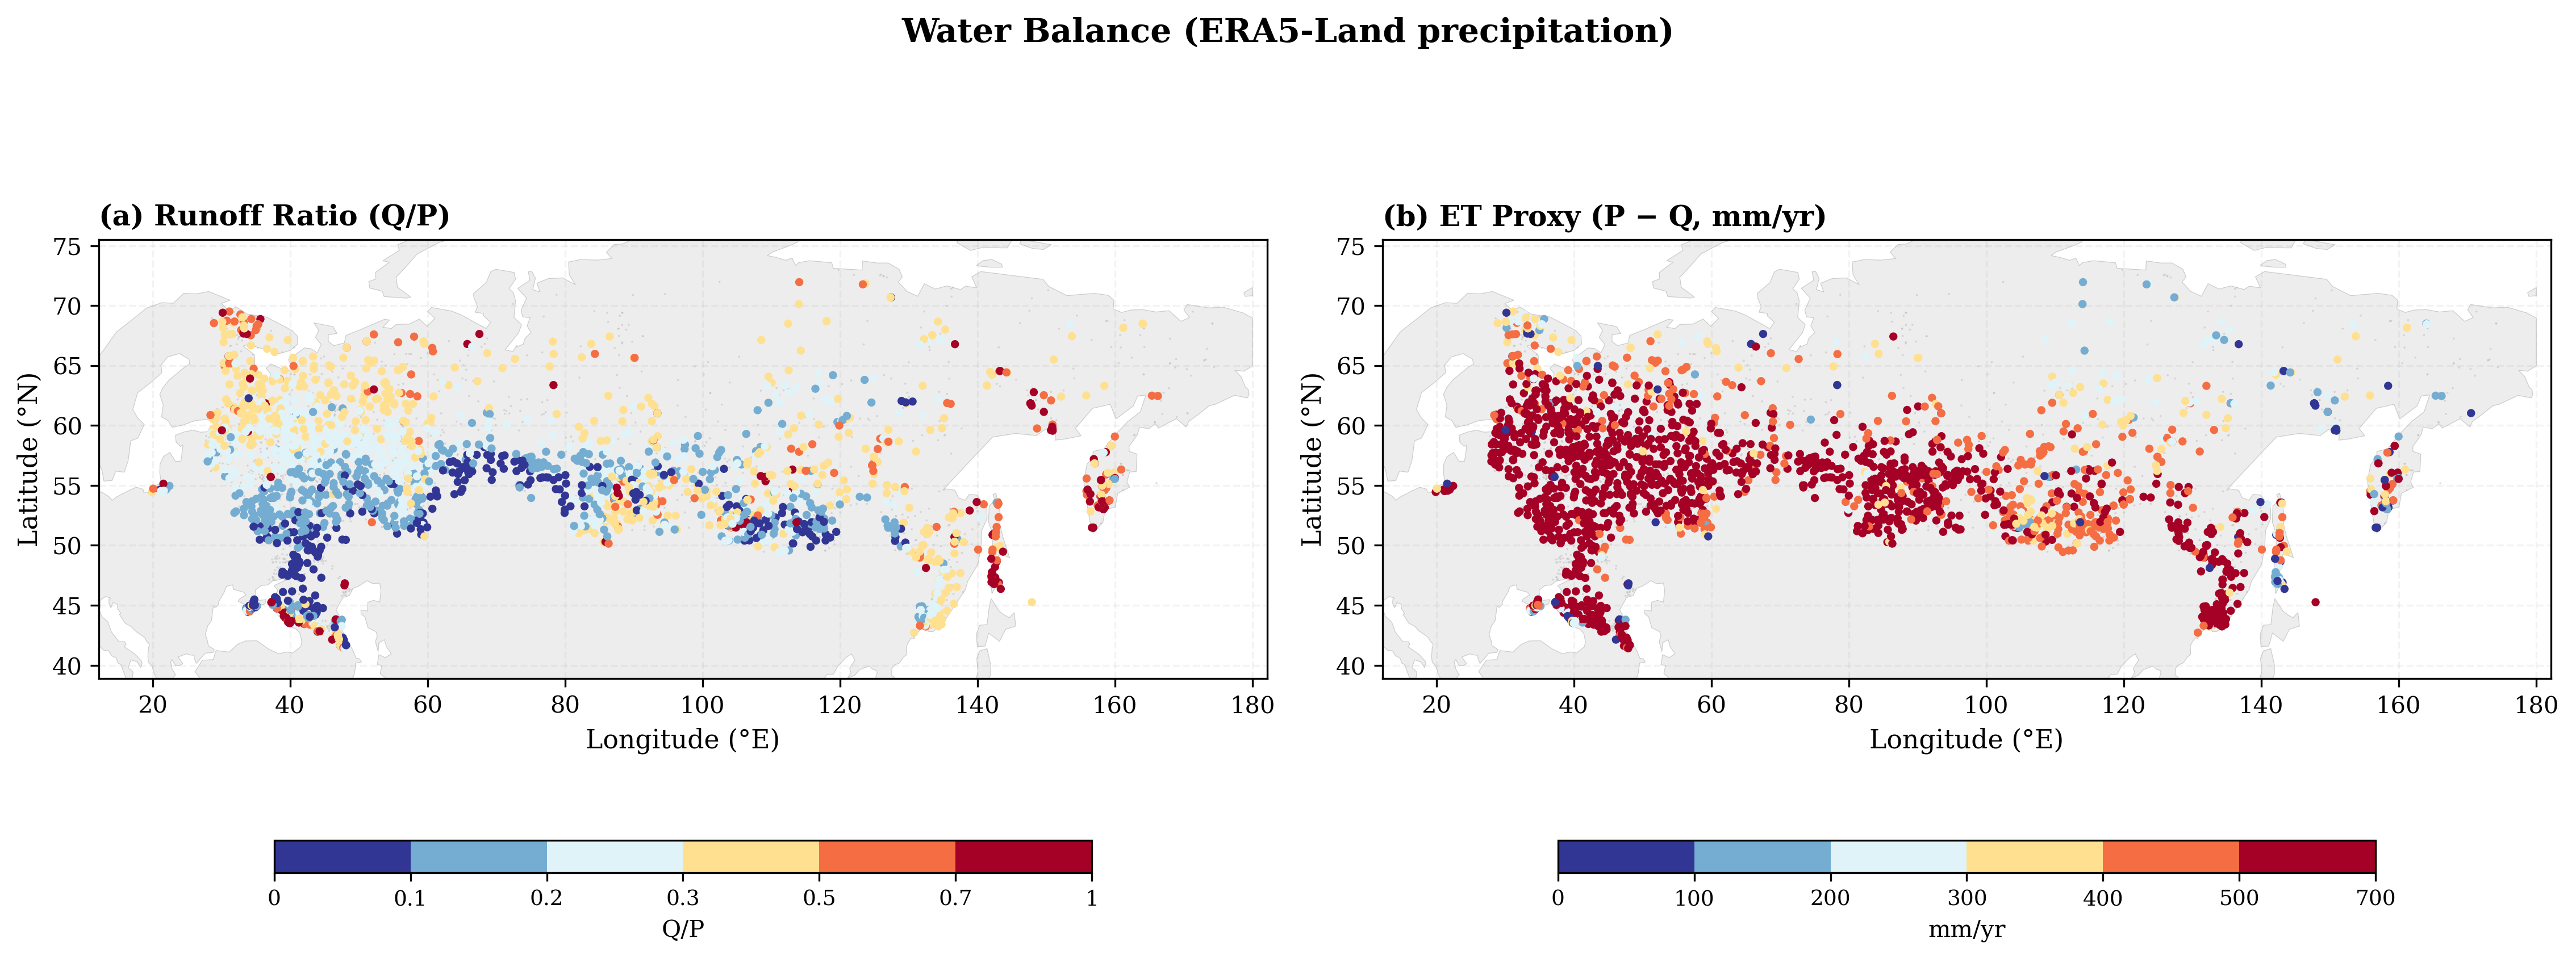
\includegraphics[width=0.95\columnwidth]{../images/fig_water_balance.png}
\caption{Water balance components across CAMELS-RU catchments: (a) runoff ratio ($Q/P$) and (b) evapotranspiration proxy ($P-Q$). ERA5-Land precipitation yields physically consistent $Q/P \leq 1$ for all catchments.}
\label{fig:water_balance}
\end{figure}

\subsection{Discharge Quality Control}

The \nhighquality high-quality discharge subset undergoes the following validation:
\begin{itemize}
    \item Physical plausibility: Zero negative discharge values after QC
    \item Temporal consistency: Cumulative sum (CUSUM) control charts applied to discharge anomalies detect mean shifts indicative of rating curve changes at 8\% of stations (flagged for metadata review)
    \item Spatial consistency: Comparison with neighboring gauges (within 100~km, similar catchment area) identifies 3\% of stations with anomalous magnitude or timing relative to neighbors
    \item Mass balance closure: Mean water balance error $<$10\% for 89\% of catchments (P$-$Q$-$ET proxy, accounting for storage)
\end{itemize}

Median data completeness: 97.5\% (2008--2023), with gaps $\leq$6 days filled by second-order polynomial interpolation (5.2\% of station-days), longer gaps retained as missing to preserve autocorrelation structure.

Figures~\ref{fig:hydro_metrics_1} and~\ref{fig:hydro_metrics_2} show spatial patterns of key hydrological signatures.
Mean annual discharge is highest in mountain headwaters and humid northern forests.
BFI is high in temperate forests (0.6--0.7) and low in permafrost regions (0.2--0.3), reflecting differences in infiltration capacity.
Half-flow date shows a latitudinal gradient from early spring snowmelt in the south to late summer in the permafrost zone.

\begin{figure}[htbp]
\centering
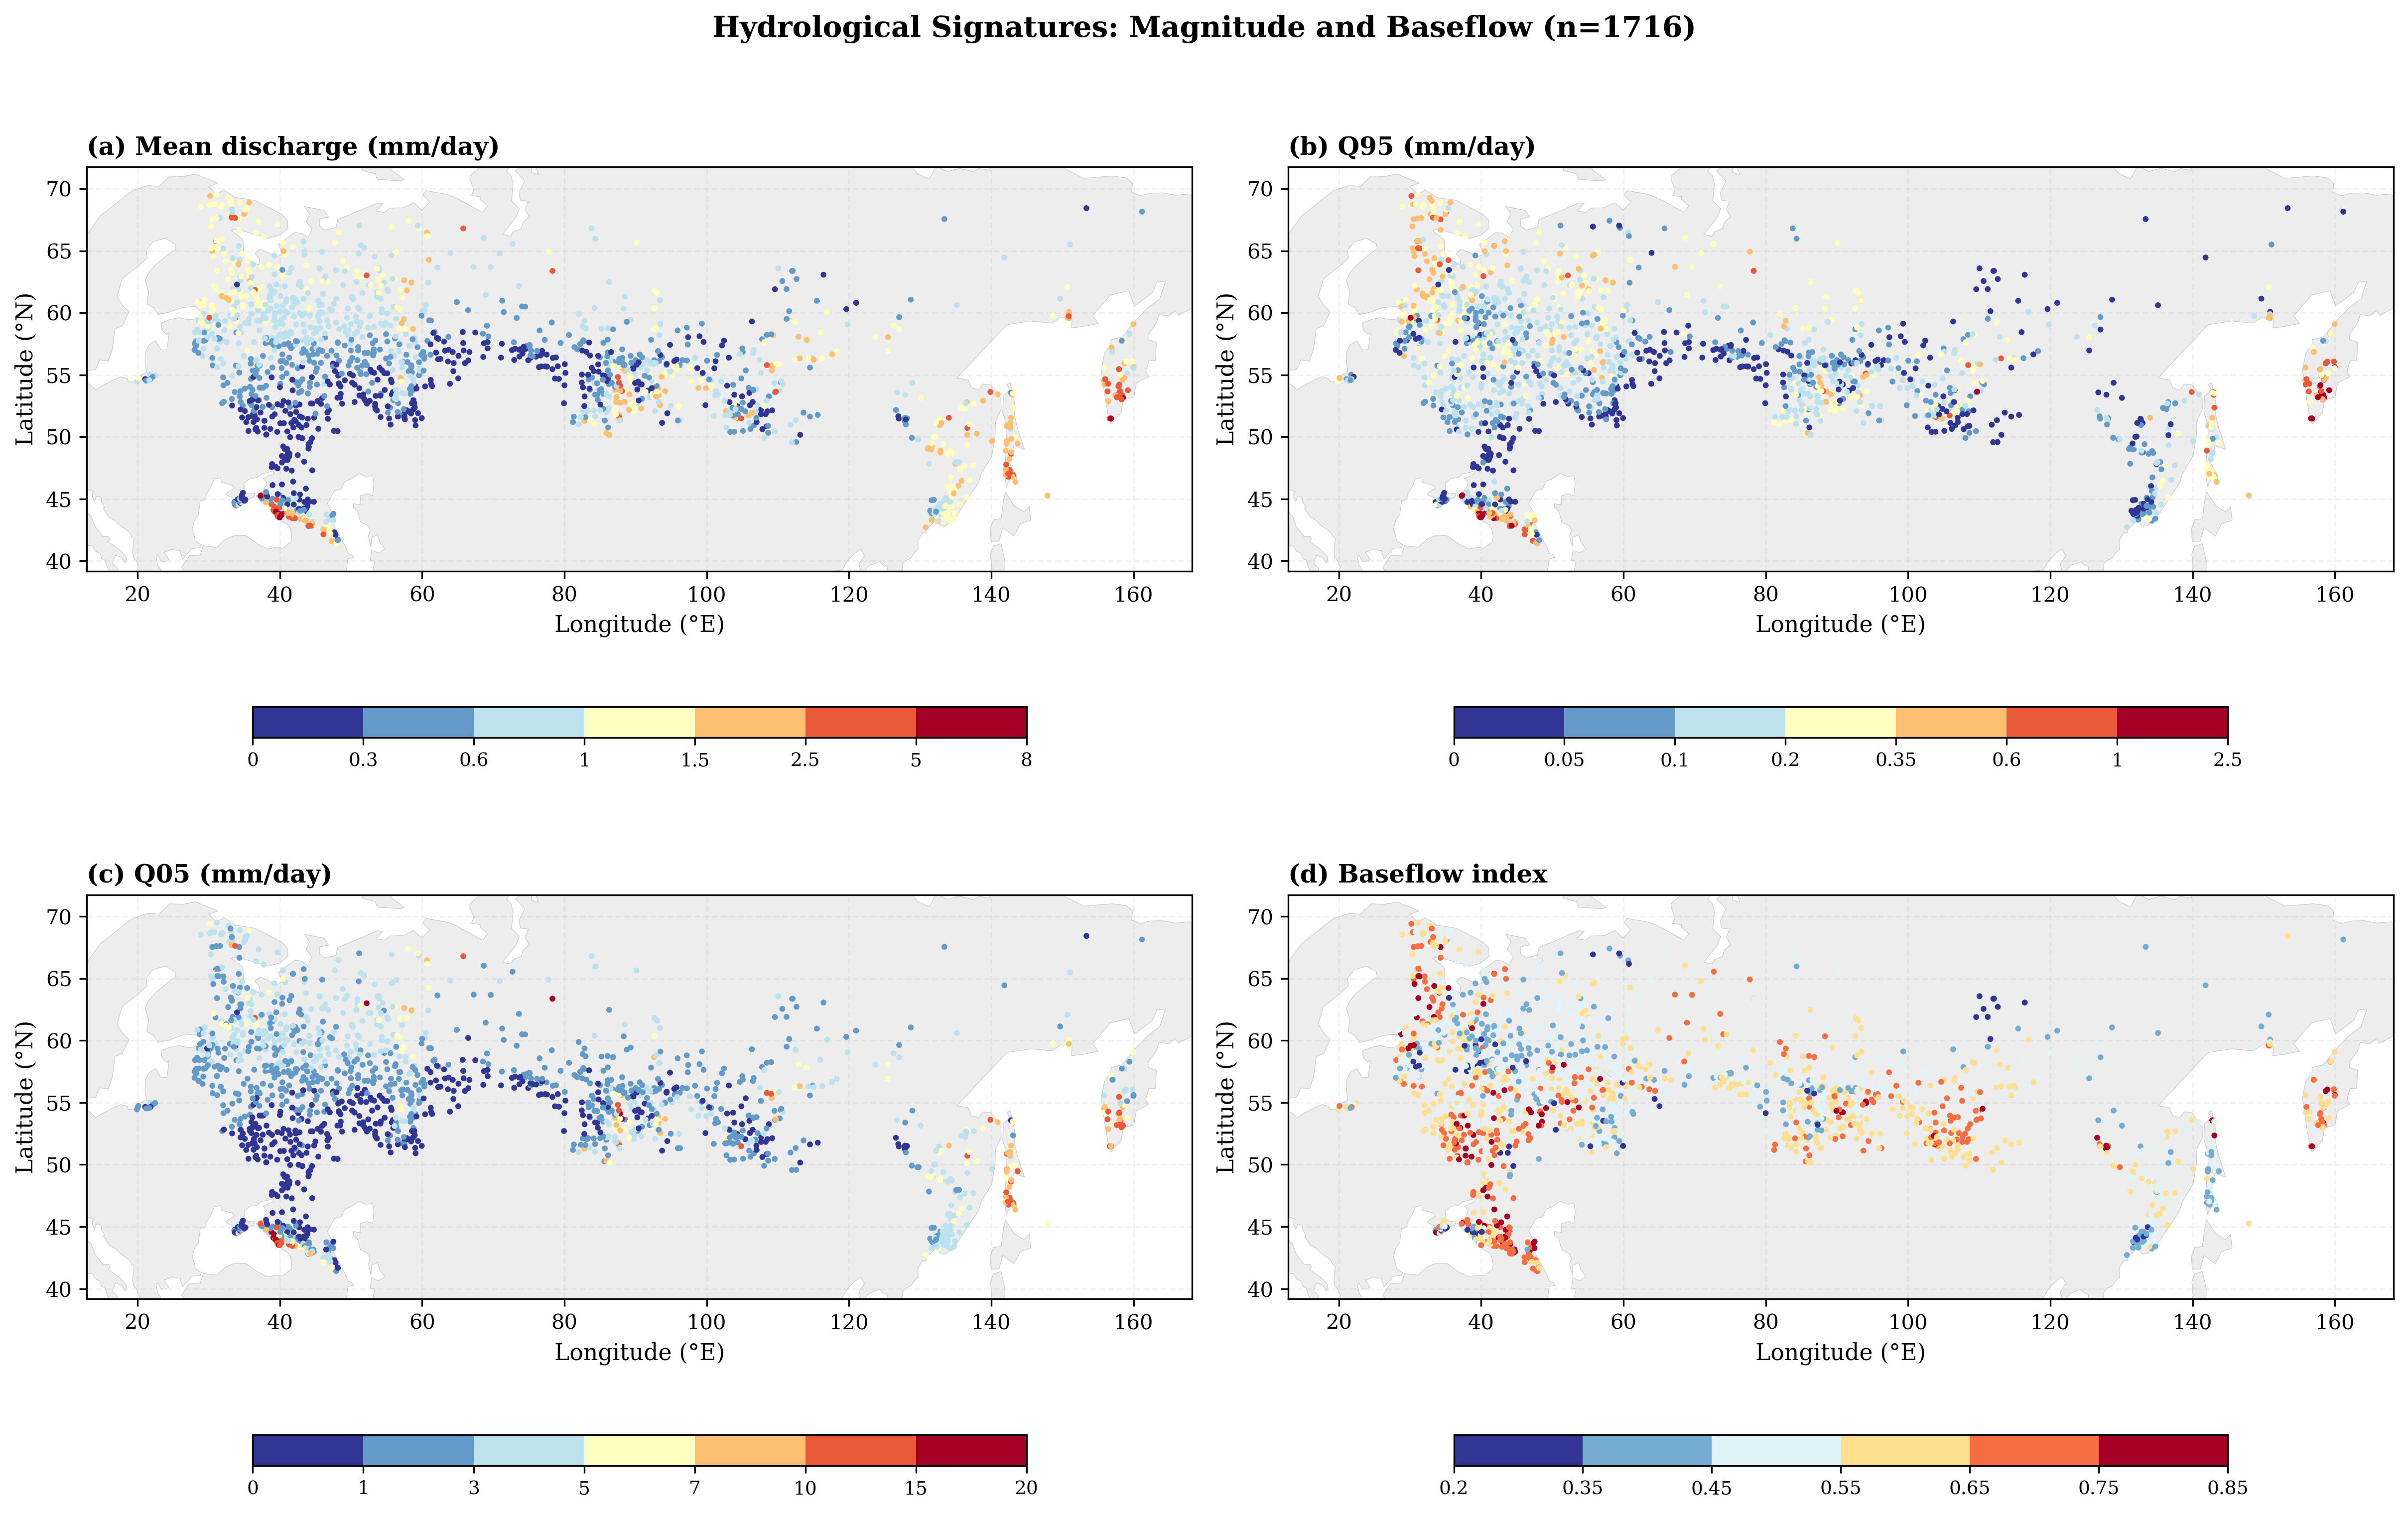
\includegraphics[width=0.95\columnwidth]{../images/fig_hydro_signatures_1.png}
\caption{Spatial distribution of magnitude and baseflow signatures: (a) mean annual discharge, (b) $Q_{95}$ (low-flow threshold), (c) $Q_{05}$ (high-flow threshold), (d) baseflow index. Color scales from low (blue) to high (red).}
\label{fig:hydro_metrics_1}
\end{figure}

\begin{figure}[htbp]
\centering
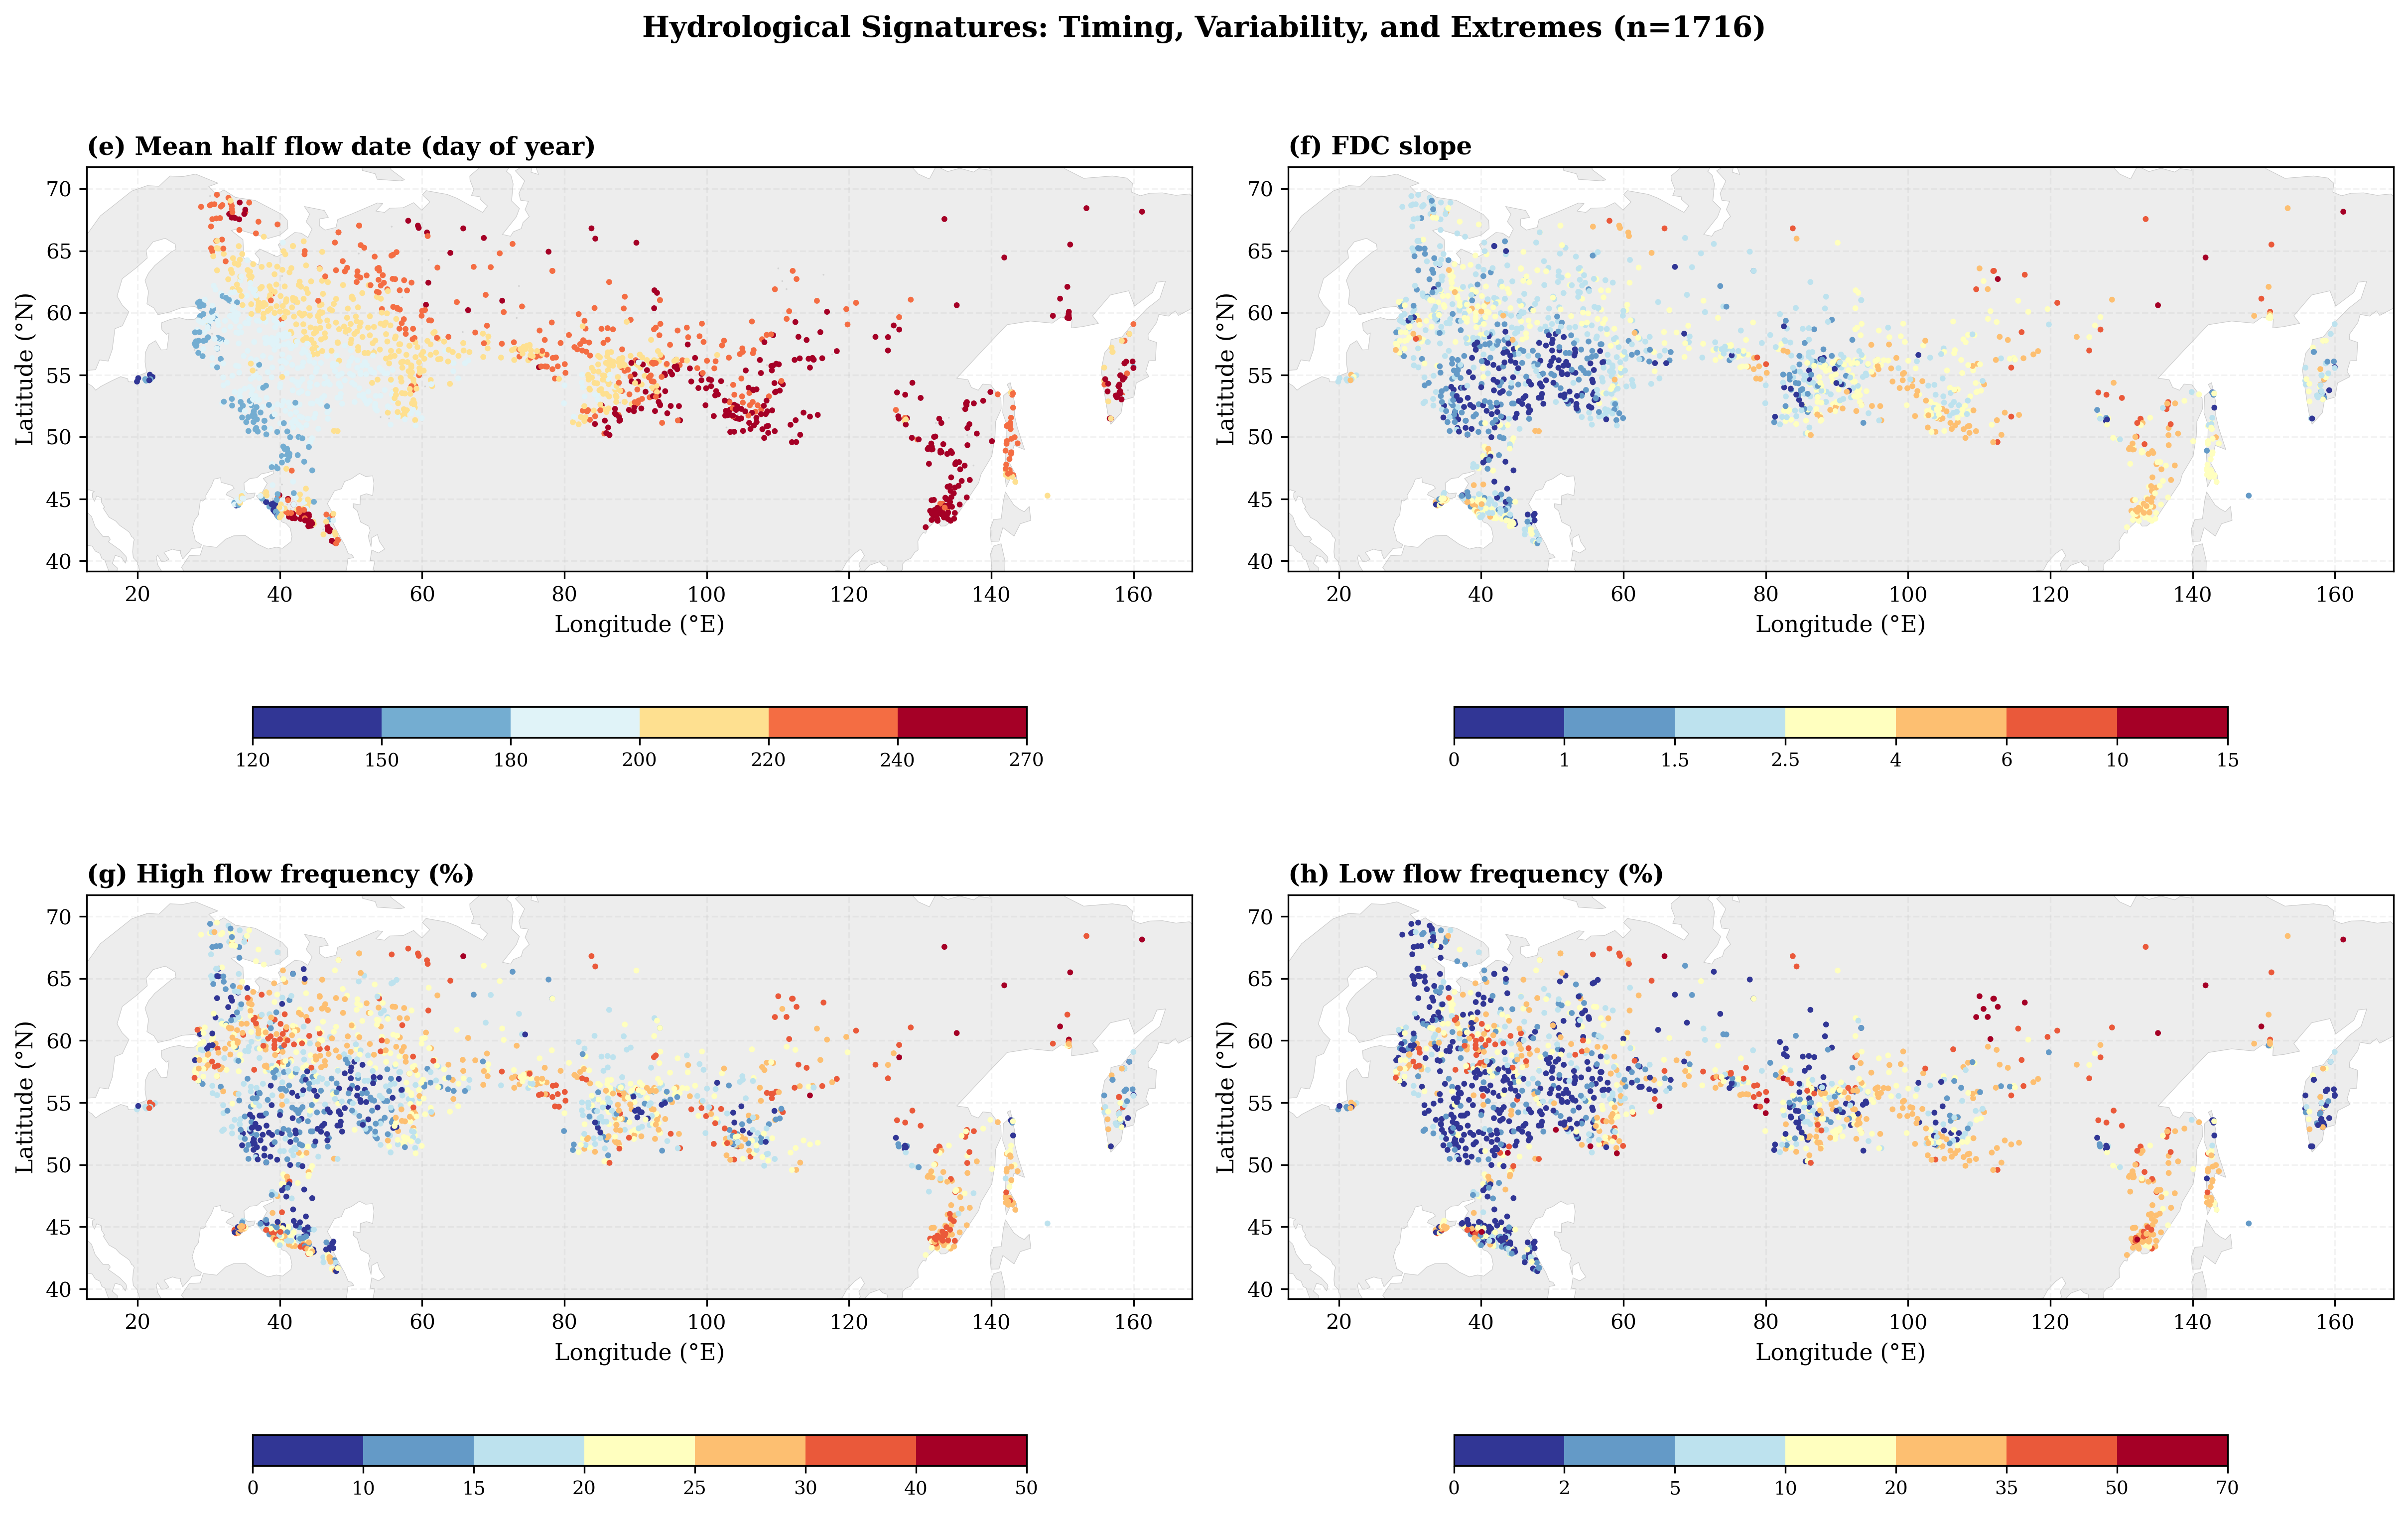
\includegraphics[width=0.95\columnwidth]{../images/fig_hydro_signatures_2.png}
\caption{Spatial distribution of timing, variability, and extreme signatures: (e) mean half-flow date (day of hydrological year), (f) FDC slope, (g) high-flow frequency, (h) low-flow frequency. Color scales from low (blue) to high (red).}
\label{fig:hydro_metrics_2}
\end{figure}

\subsection{Watershed Boundary Accuracy}

As detailed in Sect.~\ref{sec:data_sources_methods}, manual verification of all \ntotal boundaries achieved mean areal error of \meanerror against official Roshydromet data (\withinfive within 5\%, \withinten within 10\%).
The largest improvements over automated delineation occurred in:
\begin{itemize}
    \item Low-relief floodplains (West Siberian Lowland): DEM artifacts corrected using satellite imagery
    \item Permafrost regions: Subsurface flow paths verified with expert knowledge
    \item Regulated systems: Reservoir operations and diversions mapped from infrastructure databases
\end{itemize}

Independent validation using satellite-derived river widths (Global River Widths from Landsat, GRWL) shows upstream area-width scaling exponent $\beta = 0.52 \pm 0.08$, consistent with expected $\beta \approx 0.5$ from hydraulic geometry~\citep{Leopold1953}, supporting the accuracy of the delineated boundaries.


\section{Data Records}
\label{sec:data_records}

\subsection{Dataset Composition}

The dataset encompasses \ntotal catchments with delineated watersheds across Russia.
Hydrological observations include \ndischarge discharge gauging stations and \nwaterlevel water level gauges.
The high-quality subset comprises \nhighquality Grade~A gauges ($\geq$95\% completeness) during \years.
Overall, 86\% of discharge gauges meet the decent quality threshold (see Sect.~\ref{sec:data_sources_methods} for quality tier definitions).

Hydrological signatures ($N = \nsigngauges$ gauges; half-flow date: $N = \nhalfflowgauges$) span wide ranges: mean discharge \meandischarge (0.017--8.346~mm/day), BFI \meanbaseflowindex (0.210--0.903), FDC slope \meanfdcslope (0.160--13.633).

\subsection{Dataset Structure}

Table~\ref{tab:dataset_structure} summarizes the released files.
All NetCDF files include CF-compliant metadata; missing data encoded as NaN; quality flags in the discharge file distinguish observed (0), interpolated $\leq$6 days (1), suspect (2), and missing (3) values.

\begin{table}[htbp]
\centering
\caption{Dataset file structure. Total compressed size approximately 1.2~GB.}
\label{tab:dataset_structure}
\begin{tabular}{p{2.8cm}p{1.5cm}p{3.2cm}}
\toprule
\textbf{File} & \textbf{Format} & \textbf{Key variables} \\
\midrule
\texttt{boundaries.gpkg} & GeoPackage & \ntotal polygons, area, centroid, error \\
\texttt{discharge.nc} & NetCDF-4 & $Q$ (mm/d, m$^3$/s), flags; \ndischarge $\times$ 5844~d \\
\texttt{forcing.nc} & NetCDF-4 & $P$ (MSWEP), $T$, PET (ERA5-Land); \ndischarge $\times$ 5844~d \\
\texttt{attributes.csv} & CSV & 288 HydroATLAS attributes (\nattributes primary subset) \\
\texttt{signatures.csv} & CSV & \nsignatures hydro signatures \\
\texttt{water\_level/} & CSV & Daily water level (cm) for \nwaterlevel gauges \\
\bottomrule
\end{tabular}
\end{table}

\subsection{Usage Notes}

Known caveats:
\begin{itemize}
    \item Rating curve uncertainties are typically 10--20\% at high and low flows
    \item MSWEP precipitation may underestimate solid precipitation in high-latitude regions; ERA5-Land temperature and PET are reanalysis estimates with inherent model uncertainties
    \item Temporal coverage (\years, 16 years) is shorter than most CAMELS datasets, limiting multi-decadal variability analysis
    \item Gauge density is lower in remote northern and eastern regions; western European Russia is overrepresented
    \item The dataset contains nested catchments; users should account for this in spatial analyses to avoid double-counting
    \item Runoff ratio depends on precipitation product choice (see Sect.~\ref{sec:technical_validation})
\end{itemize}

The dataset is publicly available under \license license at \placeholder{[DOI: 10.XXXX/zenodo.XXXXXXX]}.
Processing code is available at \placeholder{[github.com/username/camels-ru]}.

\subsection{Limitations}
\label{sec:limitations}

\begin{itemize}
    \item \textbf{Short temporal coverage:} The 16-year record (\years) constrains multi-decadal trend analysis and captures only one phase of low-frequency climate variability.
    \item \textbf{Single DEM product:} Watershed boundaries derived from MERIT Hydro; manual verification mitigates DEM artifacts, but boundary accuracy in flat or karst terrain remains limited by the underlying elevation data.
    \item \textbf{Nested catchments:} Spatial analysis shows that the majority of gauges are nested within at least one larger catchment, with nesting depths up to 58 levels in major river systems (e.g., Ob basin). Users must account for nesting to avoid double-counting discharge or overstating sample independence.
    \item \textbf{Attribute temporal mismatch:} HydroATLAS attributes are based on circa-2000 global datasets; land cover and population density may have shifted during \years.
    \item \textbf{Stationarity assumption:} All hydrological signatures assume stationary catchment behavior, which may not hold for basins undergoing rapid land use change or permafrost degradation.
    \item \textbf{No independent discharge validation:} Discharge data are validated through internal QC and water balance consistency, but no comparison against external databases (e.g., GRDC) was performed due to limited overlap with publicly available records for Russia.
    \item \textbf{ERA5-Land circularity:} Water balance closure uses ERA5-Land precipitation, which also serves as forcing input, limiting the independence of this consistency check. Rating curve uncertainties (10--20\% at extremes) further contribute to water balance residuals.
    \item \textbf{Gauge network bias:} Arctic permafrost-dominated catchments and Pacific-draining basins are underrepresented relative to their geographic extent.
    \item \textbf{Water level data:} Water level records undergo basic QC (zero replacement, gap interpolation) but lack the automated A--F quality grading applied to discharge data. Users should assess per-gauge completeness before use.
    \item \textbf{Data source continuity:} The AIS GMVO platform, which served as the primary data source, ceased public operation in 2025. \dataset thus serves as a preservation archive for these discharge and water level records.
\end{itemize}

\subsection{Future Updates}
Planned dataset enhancements include:
\begin{itemize}
    \item Extension of temporal coverage using historical records from institute archives and OCR-digitized observation books (from the 1950s to present for a subset of gauges)
    \item Integration of additional discharge gauges with delineated watersheds
    \item Expansion of the hydropower/reservoir gauge network: additional reservoir gauges with delineated watersheds await meteorological forcing extraction and attribute computation
    \item Addition of remotely sensed variables (NDVI, snow cover extent) as dynamic attributes
\end{itemize}

\section{Conclusions}
\label{sec:conclusions}

This study presents \dataset, a large-sample hydrological dataset for \ntotal Russian catchments following the CAMELS framework, covering \years.
The key contributions are:

\textbf{1.~Dataset composition and quality control.}
\dataset consolidates \ndischarge discharge gauges and \nwaterlevel water level gauges with systematic quality control.
The high-quality subset of \nhighquality gauges achieves median data completeness of 97.5\%.
Manual expert verification of every watershed boundary (\ntotal total) achieved mean areal errors of \meanerror against official Roshydromet data.

\textbf{2.~Hydrological signatures.}
Analysis of \nsigngauges discharge records yields \nsignatures hydrological signatures spanning wide ranges: mean discharge \meandischarge (0.017--8.346~mm/day), baseflow index \meanbaseflowindex (0.210--0.903), and mean half-flow date in early May (day~\meanhalfflowday).

\textbf{3.~Meteorological forcing consistency.}
Three precipitation products (ERA5-Land: \erafiveannual; MSWEP: \mswepannual; GPCP: \gpcpannual) show pairwise daily correlations ranging from $r = \eragpcpcorr$ to $\eramsweprcorr$, with systematic differences in annual totals.
ERA5-Land yields $Q/P \leq 1$ (median \medianrunoffratio) across all catchments, though this partly reflects ERA5-Land's high-latitude wet bias rather than independent validation (see Sect.~\ref{sec:technical_validation}).

Key limitations are discussed in Sect.~\ref{sec:limitations}.
To our knowledge, \dataset is the first publicly available CAMELS-standard dataset for the Russian Federation.
The dataset enables benchmarking of hydrological models across the largest previously unrepresented landmass in the global CAMELS network.

The dataset is publicly available under \license license at \placeholder{[DOI: 10.XXXX/zenodo.XXXXXXX]}.


%% Code and data availability — Copernicus requires these specific commands.
\codedataavailability{%
The \dataset dataset (v1.0) is permanently archived on Zenodo at
\placeholder{[DOI: 10.XXXX/zenodo.XXXXXXX]} under \license license.
The dataset includes daily discharge and water level time series,
meteorological forcing (ERA5-Land, MSWEP, GPCP), physiographic attributes
(HydroATLAS), and computed hydrological signatures in NetCDF-4, GeoPackage,
and CSV formats (approximately 1.2\,GB compressed).
All processing and analysis code is publicly available at
\placeholder{[https://github.com/username/camels-ru]} under MIT license,
with pinned dependencies for full reproducibility.%
}

%% Author contributions — mandatory for Copernicus
\authorcontribution{DVA: Conceptualization, Data curation, Formal analysis, Investigation, Methodology, Software, Validation, Visualization, Writing -- original draft, Writing -- review \& editing.}

%% Competing interests — mandatory for Copernicus
\competinginterests{The author declares that there are no competing interests.}

%% Acknowledgements
\begin{acknowledgements}
The author gratefully acknowledges the Russian Federal Service for Hydrometeorology
and Environmental Monitoring (Roshydromet) for providing discharge data
through AIS GMVO, and the developers of HydroATLAS, MERIT Hydro,
ERA5-Land, MSWEP, and GPCP for making their datasets publicly
available. The broader CAMELS community is acknowledged for
establishing the framework that inspired this work.

\textit{AI disclosure:} The author used Claude (Anthropic) to assist with
code development and manuscript editing. All AI-generated content was
critically reviewed, verified against primary data sources, and revised
by the author, who takes full responsibility for the accuracy and
integrity of the work.
\end{acknowledgements}

\bibliographystyle{copernicus}
\bibliography{refs}

\end{document}
